%----------------------------------------------------------------------------------------
%	PACKAGES AND OTHER DOCUMENT CONFIGURATIONS
%----------------------------------------------------------------------------------------

\documentclass[
11pt, % The default document font size, options: 10pt, 11pt, 12pt
%twoside, % Two side (alternating margins) for binding by default, uncomment to switch to one side
english, % ngerman for German
singlespacing, % Single line spacing, alternatives: onehalfspacing or doublespacing
%draft, % Uncomment to enable draft mode (no pictures, no links, overfull hboxes indicated)
%nolistspacing, % If the document is onehalfspacing or doublespacing, uncomment this to set spacing in lists to single
%liststotoc, % Uncomment to add the list of figures/tables/etc to the table of contents
toctotoc, % Uncomment to add the main table of contents to the table of contents
parskip, % Uncomment to add space between paragraphs
%nohyperref, % Uncomment to not load the hyperref package
headsepline, % Uncomment to get a line under the header
%chapterinoneline, % Uncomment to place the chapter title next to the number on one line
consistentlayout, % Uncomment to change the layout of the declaration, abstract and acknowledgements pages to match the default layout
]{MastersDoctoralThesis} % The class file specifying the document structure

\usepackage[utf8]{inputenc} % Required for inputting international characters
\usepackage[T1]{fontenc} % Output font encoding for international characters
%\usepackage{mathpazo} % Use the Palatino font by default

\usepackage{epstopdf} % to turn my eps files into pdf
\usepackage{pgfplots}
\usepgfplotslibrary{external}
\tikzexternalize{main}

\usepackage{emptypage}

\usepackage{amsfonts}
\usepackage{amsmath}
\usepackage{mathtools} % for colon equals
\usepackage[ruled,vlined,linesnumbered]{algorithm2e} % for algorithms
\usepackage{bm} % boldface
\usepackage{enumitem} % for lists
\newcommand{\subscript}[2]{$#1 _ #2$}

\usepackage[backend=bibtex,style=ieee,natbib=true]{biblatex} % Use the bibtex backend with the authoryear citation style (which resembles APA)
\addbibresource{biblio.bib} % The filename of the bibliography
\usepackage[autostyle=true]{csquotes} % Required to generate language-dependent quotes in the bibliography
\setlength\parindent{0pt} % no-indents

\usepackage{tikz}
\usepgfplotslibrary{external} 
\tikzexternalize

\usepackage[dvipsnames]{xcolor}

%----------------------------------------------------------------------------------------
%	MATH SHORTCUTS
%----------------------------------------------------------------------------------------

% Define some commands to keep the formatting separated from the content 
\newcommand{\E}{\mathbb{E}}
\newcommand{\Var}{\mathrm{Var}}
\newcommand{\Cov}{\mathrm{Cov}}
\newcommand*{\B}[1]{\mathbf{#1}}
\DeclareMathOperator*{\argmin}{arg\,min} % thin space, limits underneath in displays
\DeclareMathOperator*{\argmax}{arg\,max} % thin space, limits underneath in displays

\newcount\colveccount
\newcommand*\colvec[1]{
        \global\colveccount#1
        \begin{bmatrix}
        \colvecnext
}
\def\colvecnext#1{
        #1
        \global\advance\colveccount-1
        \ifnum\colveccount>0
                \\
                \expandafter\colvecnext
        \else
                \end{bmatrix}
        \fi
}

\def\x{\mathbf{x}} % Small x boldface
\def\X{\mathbf{X}} % Capital X boldface
\def\D{\mathcal{X}} % mathcal X the domain D
\def\Da{\mathcal{D}} % mathcal D the DAta D
\def\N{\mathcal{N}} % Normal distribution
\def\f{\mathbf{f}} % Small f boldface
\def\y{\mathbf{y}} % Small y boldface
\def\param{\bm{\theta}} % bold theta

\newcommand{\keyword}[1]{\textbf{#1}}
\newcommand{\tabhead}[1]{\textbf{#1}}
\newcommand{\code}[1]{\texttt{#1}}
\newcommand{\file}[1]{\texttt{\bfseries#1}}
\newcommand{\option}[1]{\texttt{\itshape#1}}

%----------------------------------------------------------------------------------------
%	MARGIN SETTINGS
%----------------------------------------------------------------------------------------

\geometry{
	paper=a4paper, % Change to letterpaper for US letter
	inner=3.5cm, % Inner margin
	outer=3.5cm, % Outer margin
	bindingoffset=0cm, % Binding offset
	top=4cm, % Top margin
	bottom=5cm, % Bottom margin
	%showframe, % Uncomment to show how the type block is set on the page
}

%----------------------------------------------------------------------------------------
%	THESIS INFORMATION
%----------------------------------------------------------------------------------------

\thesistitle{Constrained Bayesian Optimization} % Your thesis title, this is used in the title and abstract, print it elsewhere with \ttitle
\supervisor{Dr. Georgios \textsc{Karagiannis}} % Your supervisor's name, this is used in the title page, print it elsewhere with \supname
\degree{Bachelor of Mathematics} % Your degree name, this is used in the title page and abstract, print it elsewhere with \degreename
\author{} % Your name, this is used in the title page and abstract, print it elsewhere with \authorname
\subject{Mathematical Sciences} % Your subject area, this is not currently used anywhere in the template, print it elsewhere with \subjectname
\keywords{} % Keywords for your thesis, this is not currently used anywhere in the template, print it elsewhere with \keywordnames
\university{Durham University} % Your university's name and URL, this is used in the title page and abstract, print it elsewhere with \univname
\department{Department of Mathematical Sciences} % Your department's name and URL, this is used in the title page and abstract, print it elsewhere with \deptname
\group{Research Group Name} % Your research group's name and URL, this is used in the title page, print it elsewhere with \groupname
\faculty{Faculty Name} % Your faculty's name and URL, this is used in the title page and abstract, print it elsewhere with \facname

\AtBeginDocument{
\hypersetup{pdftitle=\ttitle} % Set the PDF's title to your title
\hypersetup{pdfauthor=\authorname} % Set the PDF's author to your name
\hypersetup{pdfkeywords=\keywordnames} % Set the PDF's keywords to your keywords
}

\begin{document}

\frontmatter % Use roman page numbering style (i, ii, iii, iv...) for the pre-content pages

\pagestyle{plain} % Default to the plain heading style until the thesis style is called for the body content

%----------------------------------------------------------------------------------------
%	TITLE PAGE
%----------------------------------------------------------------------------------------

\begin{titlepage}
\begin{center}

\vspace*{.06\textheight}
{\scshape\LARGE \univname\par}\vspace{1.5cm} % University name

\HRule \\[0.4cm] % Horizontal line
{\huge \bfseries \ttitle\par}\vspace{0.4cm} % Thesis title
\HRule \\[1.5cm] % Horizontal line

 
\begin{minipage}[t]{0.4\textwidth}
\begin{flushleft} \large
\emph{Author:}\\
{Adam \textsc{Howes}} % Author name - remove the \href bracket to remove the link
\end{flushleft}
\end{minipage}
\begin{minipage}[t]{0.4\textwidth}
\begin{flushright} \large
\emph{Supervisor:} \\
{\supname} % Supervisor name - remove the \href bracket to remove the link  
\end{flushright}
\end{minipage}\\[3cm]
 
\vfill

\large \textit{Submitted in partial fulfilment of the requirements\\ for the degree of \degreename}\\[0.3cm] % University requirement text
 
\vfill

{\large \today}\\[4cm] % Date
%\includegraphics{Logo} % University/department logo - uncomment to place it
 
\vfill
\end{center}
\end{titlepage}

%----------------------------------------------------------------------------------------
%	DECLARATION PAGE
%----------------------------------------------------------------------------------------

\begin{declaration}
\addchaptertocentry{\authorshipname} % Add the declaration to the table of contents
\noindent I, Adam \textsc{Howes}, declare that this project titled, \enquote{\ttitle} is a result of my own work except where it forms an assessment based on group project work. In the case of a group project, the work has been prepared in collaboration with other members of the group. Material from the work of others not involved in the project has been acknowledged and quotations and paraphrases suitably indicated. Code for all figures and experiments in this project is available at \url{https://github.com/athowes/cbo}.\\
 
\noindent Signed:\\
\rule[0.5em]{25em}{0.5pt} % This prints a line for the signature
 
\noindent Date:\\
\rule[0.5em]{25em}{0.5pt} % This prints a line to write the date
\end{declaration}

\cleardoublepage

%----------------------------------------------------------------------------------------
%	ABSTRACT PAGE
%----------------------------------------------------------------------------------------

\begin{abstract}
\addchaptertocentry{\abstractname} % Add the abstract to the table of contents
This project introduces the reader to Bayesian optimization, a sequential algorithm for the global optimization of expensive-to-evaluate, black-box functions. We also present some recent research in extending Bayesian optimization to deal with constrained optimization problems.

\vspace*{0.2\textheight}

\vspace*{0.2\textheight}

\noindent\enquote{\itshape Is this Bayesian? You know I'm a strict Bayesian, right?}\bigbreak

\hfill \href{https://twitter.com/ML_Hipster}{@ML{\_}Hipster}

\end{abstract}

%----------------------------------------------------------------------------------------
%	ACKNOWLEDGEMENTS
%----------------------------------------------------------------------------------------

\begin{acknowledgements}
\addchaptertocentry{\acknowledgementname} % Add the acknowledgements to the table of contents
Thanks to Georgios for his guidance and support throughout.
\end{acknowledgements}

%----------------------------------------------------------------------------------------
%	LIST OF CONTENTS/FIGURES/TABLES PAGES
%----------------------------------------------------------------------------------------

\tableofcontents % Prints the main table of contents

%\listoffigures % Prints the list of figures
%
%\listoftables % Prints the list of tables

%----------------------------------------------------------------------------------------
%	THESIS CONTENT - CHAPTERS
%----------------------------------------------------------------------------------------

\mainmatter % Begin numeric (1,2,3...) page numbering

\pagestyle{thesis} % Return the page headers back to the "thesis" style

% Include the chapters of the thesis as separate files from the Chapters folder

% Chapter 1

\chapter{Background} % Main chapter title

\label{Chapter1} % For referencing the chapter elsewhere, use \ref{Chapter1} 

%----------------------------------------------------------------------------------------

\section{Problem definition}

Optimization, the act of finding the best action in a given situation, is both a ubiquitous problem and one of a great importance. Mathematically, the \textit{global} optimization of a real-valued function $f:\D \to \mathbb{R}$ aims to find a minimizer $\x^\star$ (there may be more than one) in the search space $\D$, such that:
%
\begin{equation} \label{eq:1.1}
\x^\star = \argmin_{\x\in\D} f(\x)
\end{equation}
%
Considering $g(\x) = -f(\x)$ shows, as would be expected, that maximization is equivalent. The function $f$ to be optimized is referred to as the \textit{objective function}. In contrast to local optimization, global optimization requires that $f(\x^\star) \leq f(\x)$ for \textit{all} $\x \in \D$ rather than only in some neighbourhood about $\x^\star$. In this project, we assume that the search space $\D$ is a compact subset of  $\mathbb{R}^d$ where $d \in \mathbb{N}$.

This problem, given by equation \ref{eq:1.1}, is the subject of a vast array of scientific literature. In practise, the objective function $f$ may additionally have the following challenging properties P1 - P4:
%
\begin{enumerate}[label={P}{\arabic*}]
\item{ \label{itm:p1}
\textbf{Non-linear, non-convex}: In general, the objective function cannot be assumed to be linear or, more broadly, convex. The extensive fields of linear programming and convex optimization study these cases respectively. \citet{rockafellar1993lagrange} famously describes that in truth the ``great watershed in optimization'' lies between the difficulty of the convex and non-convex cases.
}
\item{ \label{itm:p2}
\textbf{Black-box}: A function is called \textit{black-box} if it can only be viewed in terms of its inputs and outputs. If $f$ is black-box then it does not have analytic form or derivatives, such as the gradient $\nabla f$ or Hessian $\mathbf{H}$, which can be reasoned about and, in particular, used in the search for $\B{x}^*$. As \citet{vizier} note in their paper about Google's in-house black-box optimizer:
%
\begin{quotation}
``Any sufficiently complex system acts as a black-box when it becomes easier to experiment with than to understand''
\end{quotation}
%
To this end, they suggest that as the systems we create, and hope to optimize, increase in complexity, black-box optimization techniques will become increasingly important. For problems with this property, optimization may only proceed by querying $f$ point-wise at inputs $\x\in\D$ in order to learn about its behaviour.
}
\item{ \label{itm:p3}
\textbf{Expensive to evaluate}: The sampling procedure is computationally, economically or otherwise prohibitively expensive. Most prevalently the objective function is time-consuming to evaluate. For example, when tuning the hyper-parameters of a machine-learning model, each function evaluation is potentially very time-intensive as it corresponds to training and evaluating the performance of the primary model \citep{snoek2012practical}. That being said, there are many examples of more general costs. In chemistry, in order to optimize the yield of a reaction, evaluating the objective function involves potentially resource-intensive and laborious experiments. No matter the resource in question, practitioners have finite budgets and, as a result, may only be able to afford relatively few function evaluations. Often it is specified that the number of function evaluations which can be afforded is $N$- which we will take to be the case in this project. More general formulations may, among other considerations, take into account the variable costs of sampling at different locations \cite{snoek2012practical}.
}
\item{ \label{itm:p4}
\textbf{Noisy}: When $f$ is evaluated at $\x$, the value returned $y$ is contaminated by noise $\epsilon$, assumed to be Gaussian with zero mean and variance $\sigma^2$ such that $y = f(\x) + \epsilon$. Problems of this sort are described as \textit{stochastic programming} problems.
}
\end{enumerate}

This project will begin in Chapters \ref{Chapter1}, \ref{Chapter2} and \ref{Chapter3} with an introduction to \textit{Bayesian optimization}, which is a state-of-the-art method intended for optimizing objective functions with the above properties. 

Bayesian optimization and related approaches have a rich history. Their popularity among practitioners and researchers is steadily increasing \cite{shahriari2016taking}. 

\newpage

\section{Pragmatic aims} \label{sec:prag}

Solving equation \ref{eq:1.1}, namely finding a minimizer $\x^\star$, with the additional challenges \ref{itm:p1}-\ref{itm:p3} is a difficult undertaking (leaving \ref{itm:p4} a moment). If it is assumed that $f$ is Lipschitz-continuous, that is
%
\begin{equation}
\nonumber \exists \, l \geq 0 \quad\mathrm{s.t.}\quad \forall \, \x, \x' \in \D, \quad \lvert f(\x) - f(\x') \rvert \leq l \lvert \x - \x' \rvert,
\end{equation}
%
then it can be guaranteed that a minimizer $\x^\star$ exists \citep{horst2013handbook}. However, finding it in general is not possible using a finite number of function evaluations \citep{lizotte}. Even guaranteeing a solution evaluates to within $\epsilon$ of the true maximum $f(\x^\star)$, which we will call \textit{$\epsilon$-optimality}, requires a minimax approach where a grid of samples are made with resolution proportional to $\epsilon$ \citep{betro1991}. Sometime called the ``curse of dimensionality'', the number of points in such a grid scales exponentially with the dimension $d$, which quickly becomes impractical even in low dimensions due to property \ref{itm:p2}. The situation is only made worse if evaluating the objective function is also noisy, \ref{itm:p4}. For this reason, some clarification is required on the aims of optimization in the face of what is considerable adversity. 

\citet{lizotte} proposes a principle of perseverance, noting that although the problem is difficult that doesn't make it go away. The world is full of difficult optimization problems that we would still like to make progress on. The good news is that overwhelmingly the task is not all-or-nothing. That is, suboptimal solutions may be perfectly viable if the contextual performance difference is small. In some situations, perhaps when sampling has a meaningful financial cost for example, a cheap suboptimal solution may even be preferred. Furthermore, the previous minimax approach pays a high price to insure against worst-case, pathological scenarios which may not be very plausible in reality \citep{brochu2010interactive}. 

These considerations motivate a ``practical'' \citep{lizotte} or ``average-case'' \citep{streltsov1999non} approach, where the focus is in finding a ``good'' solution or converging on a minimizer $\x^\star$ in few evaluations, rather than in making theoretical guarantees about optimality. This is the philosophy that we will adopt during this project.

\section{Sample designs} \label{sampledesigns}

How, then, should points be queried to efficiently learn about $\x^\star$ so that the above aims can be met?

We first present two relatively naive strategies: \textit{grid-search} and \textit{random-search}. These approaches directly select a set of points, called a sample design, to be evaluated. Grid-search is previously mentioned above, where a dense grid was used by \citet{betro1991} to ensure $\epsilon$-optimality. Of course, the resolution need not be so high. More generally, in a grid-search samples are taken spaced evenly throughout the domain $\D$ at a resolution appropriate to the optimization budget. Although the whole domain is superficially covered, if few function evaluations can be afforded then this coverage is too sparse to reliably locate a minimizer. Meanwhile, random-search simply chooses inputs in the domain $\D$ to evaluate at random.

Perhaps counter-intuitively, \citet{bergstra2012random} show that in some sense random-search actually performs more efficiently than grid-search. In particular, grid-search performs very poorly when the objective function $f$ has a low effective dimensionality. This is because multiple sample points have the same value when collapsed down onto any dimension. Looking at it another way, if one of the dimensions has little impact then in a grid-search many samples are entirely wasted - without learning \textit{anything} about the other dimensions. That being said, random-search is also severely flawed: complete randomness lends itself to clumps of points and large areas left empty. 

One way of overcoming these problems is to use a space-filling, but still random, design such as the \textit{latin-hypercube} \cite{lectures}. Latin-hypercube designs generalize the latin-square, which is a grid with exactly one sample in each column and each row, to arbitrary dimension. This avoids the problem of collapsing, from which grid-search suffers. Figure \ref{fig:1i} gives an example of the usage of each of grid-search, random-search and latin-hypercube sampling on a two dimensional objective function. 

\begin{figure}
\centering
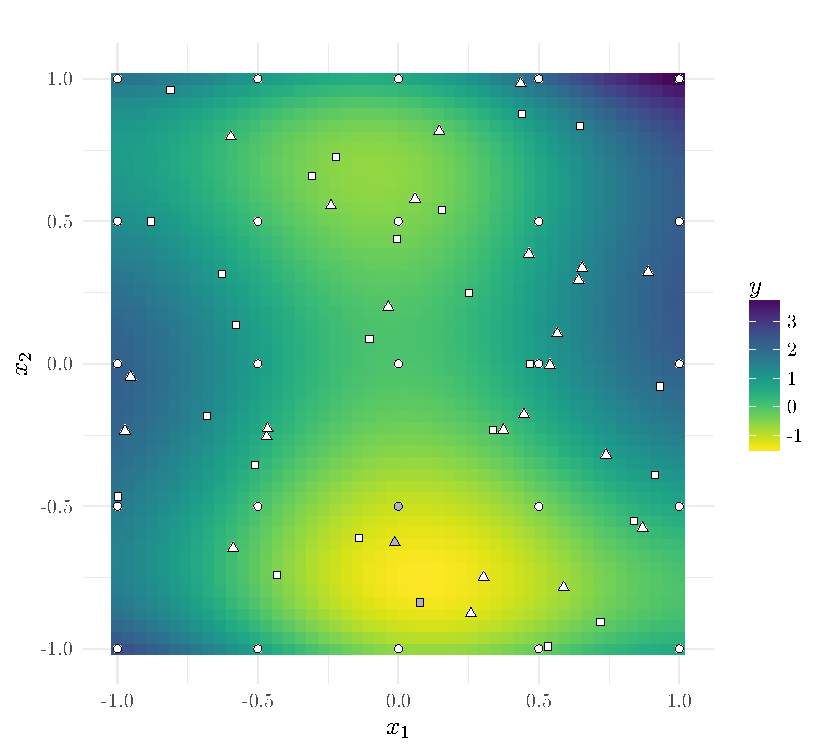
\includegraphics[scale=1]{fig1i.pdf}
\begin{tabular}{ l | l c c }
              & Symbol & $y_{\mathrm{min}}$ & $(x_1, x_2$)\\ \hline
  Grid-search & Circles & -1.050 & $(0.000, -0.500)$\\
  Random-search & Triangles & -1.322 & $(0.131, -0.638)$\\
  Latin-hypercube & Squares & -1.382 & $(0.078 -0.837)$\\
\end{tabular}
\caption[width=\linewidth]{Density plot of modified two-dimensional camel function $y = (4 - 2.1x_1^2 + 0.3x_1^4)x_1^2 + (x_1+0.6)x_2 + (-4+4x_2^2)x_2^2$ on the square $x_1 \in [-1,1], x_2 \in [-1,1]$. 25 points sampled from each of grid-search, random-search and latin-hypercube sampling; minimum found by each method shown in grey. True global minimum is -1.470 at $(0.094, -0.747)$.} \label{fig:1i} 
\end{figure}

\section{Models \& trade-offs}

Although there are many more complicated and arguably better sample designs than the ones described above, it is intuitively clear that any such strategy is suboptimal: information gained during the search is not used to better inform the next decision. Rather than choose all the points at once it makes sense instead to consider a sequential decision making problem where at each stage a point is carefully chosen to be evaluated next. The same philosophy is true of many situations. It would be unwise to require students starting at Durham to choose their modules for first, second and third year all at once as their preferences will surely change as they learn more.

So, how can this information be used? It is important to note that in order to learn about the behaviour of the objective function where it has not been specifically sampled we must make some assumptions about how the data we have may be extrapolated. In particular, we assume that points close in input are to some extent close in output. In other words, that $f$ is somewhat smooth. Making assumptions, like this one, about the nature of the objective function is helpful if those assumptions are right. If they are not too strong or restrictive, then \textit{on-average} they will be right \cite{blog}. This is the foundational idea of the model-based approach to optimization, in which statistical inference can be used to aid in the search process.

Assuming that the objective function $f$ is smooth, there are two types of location which should be the focus of the search. Firstly, sampling in uncertain regions, not near to any previous evaluations, will provide helpful information about the global behaviour of the objective function. On the other hand, sampling in promising regions, near to previous low evaluations, will allow solutions to be refined locally. We will term these two contrasting ideas as \textit{global search} and \textit{local search}, respectively. This is slightly non-standard terminology, the reason for which will be explained shortly in section \ref{sec:bandits}.

Good strategies then must appropriately balance global search and local search. Too great a focus on global search leads to the optimization never converging on a solution. Conversely, too great a focus on local search tends to locate local rather than global minimizers.

The sample designs given in section \ref{sampledesigns} are all examples of strategies which neglect local search. Once they find a promising location they would be better served to invest more of their attention in that area - so that they may informally ``drill-down'' \cite{lectures} to a better solution.

On the other hand, for example techniques which iteratively alter solutions in order to get an idea of the gradient, with the idea being to move in the direction of greatest decrease, have too great a focus on local-search. A ball on the surface of figure \ref{fig:1i} will roll into the local minima (rather than the global minima) if is placed too close - in the so-called \textit{basin of attraction}. In practise this problem may be remedied by random restarts, i.e. repeating the search a number of times with the ball placed randomly each time. However, this alteration is not viable in view of property \ref{itm:p4}. The fact that the local minima is a global minima when the objective function is convex is what makes convex optimization significantly more approachable than the general case.

\newpage

\section{Bayesian optimization} \label{BO}

Bayesian optimization \citep{kushner1964new} \citep{mockus1974bayesian} aims at addressing the optimization of objective functions with the above properties \ref{itm:p1}-\ref{itm:p3} and possibly \ref{itm:p4}. It is a sequential, model-based optimization algorithm which learns from all available observations to make better informed choices about the next point to query. The algorithm is detailed in algorithm \ref{algo:1} and has two key components: the statistical \textit{emulator} and the \emph{acquisition function}. 

As $f$ is black-box, there is uncertainty about its true value where it has not been directly evaluated (and when $f$ is noisy then even at evaluated points as well). It is theoretically justified \citep{cox} that Bayesian probability theory is a rational way to reason about such uncertain states of knowledge. Prior beliefs about the objective function and data-generation mechanism may be encapsulated with an explicit, probabilistic, statistical model. 

\begin{figure}
\begin{flushleft} \hspace{25pt} (a) Stage $n=1$ \end{flushleft}
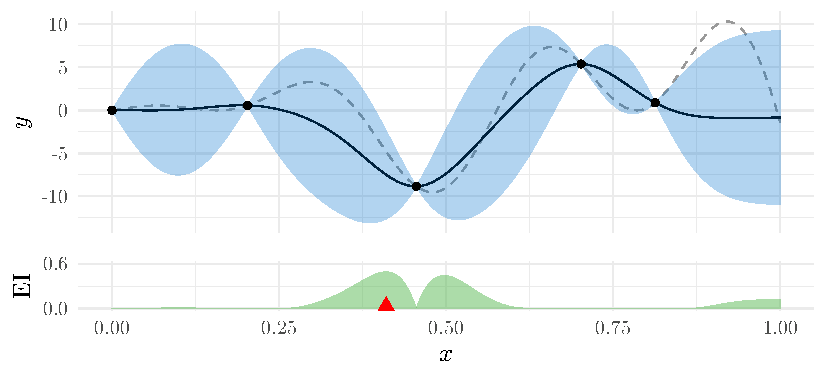
\includegraphics[scale=1]{fig1iia.pdf}
\begin{flushleft} \hspace{25pt} (b) Stage $n=2$ \end{flushleft}
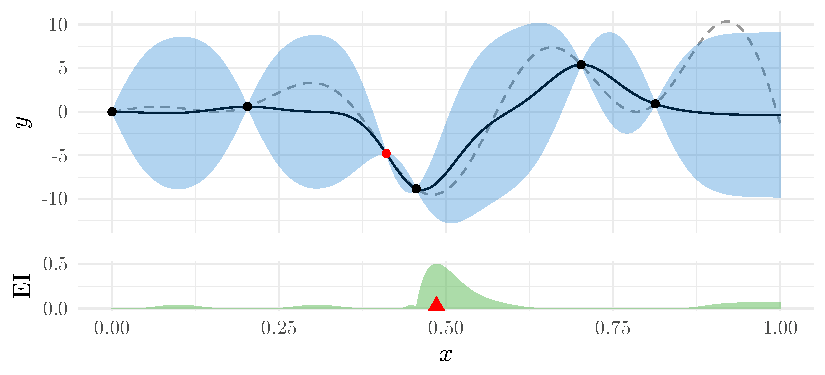
\includegraphics[scale=1]{fig1iib.pdf}
\centering
\caption{A two-stage example run of Bayesian optimization. Objective function $f(x) = 10x(\sin(10x) + \cos(20x))$ is shown as the dahsed grey line in both (a) and (b). The mean of the Gaussian process emulator, i.e. the surrogate function, at each stage is shown as the solid black line. Uncertainty about the objective function is shown as the light-blue point-wise $95\%$ confidence region. The initial data-set $\Da_0$ is five points and their noise-free evaluations generated by latin hyper-cube sampling. The acquisition function is shown in green, with its maximum at each stage shown by the red arrow. Here we use the one particular acquisition function, expected improvement (EI), which will be properly introduced in Chapter \ref{Chapter3}. The acquisition function maximum in (a) is shown evaluated as the red circle in (b).} \label{fig:1ii}
\end{figure}

This probabilistic model is known as an emulator \cite{lectures}. It should behave similarly to the objective function $f$, but be much cheaper to work with. The emulator provides a predictive distribution for $f$ evaluated at new inputs. The mean of this distribution may be used as a \textit{surrogate} for the objective function and the variance allows for uncertainty quantification.  When data $\{\x, y\}$ is observed then the model can be sequentially updated and refined, using Bayes' rule. 

Typically the emulator used is a \textit{Gaussian process}, which is a convenient and flexible model for this purpose. We will introduce Gaussian processes and their role in Bayesian optimization in more detail in Chapter \ref{Chapter2}.  

To guide the search for a global minimizer, the emulator is leveraged by an acquisition function, sometimes also called an in-fill function. It is a function of the state of the optimization at the current stage $n$, i.e. all of the data which is available and the Gaussian process emulator to the objective function $f$, which returns a suggestion of the next point to sample $\x_n$. This function automatically balances the trade-off between global and local search. Many possible acquisition functions have been proposed in the literature. This will be explored in more depth in Chapter \ref{Chapter3}. 

% Algorithm: General Bayesian Global Optimization 
\begin{algorithm}
\SetAlgoLined
\textbf{input} objective function $f$, acquisition function $\alpha$, initial dataset $\Da_0$\;
 \For{$n = 1, 2, \ldots, N$}{
  Fit Gaussian process to dataset at stage $n$, $\Da_{n-1}$\;
  Maximize acquisition function $\alpha$ over Gaussian process to propose next point to sample, $\x_{n}$\;
  Query objective function $f$ at $\x_{n}$, returning $y_{n} = f(\x_{n}) + \epsilon$\;
  Augment dataset $\Da_{n} = \Da_{n-1} \cup \{\x_{n}, y_{n}\}$\;
 }
Fit Gaussian process to complete dataset $\Da_{N}$\;
\Return{\textrm{recommendation} $\x^-$}\;
\vspace{5pt}
\caption{Bayesian optimization algorithm} \label{algo:1}
\end{algorithm}

Figure \ref{fig:1ii} gives a toy example of the use of Bayesian optimization for a one-dimensional objective function, illustrating stages $n=1,2$ in algorithm \ref{algo:1}. In this example, the optimization begins with an already available data-set $\Da_0$ which is used to build the inital Gaussian process emulator. It has been suggested that in general a small number of points, depending on the dimension, should be sampled prior to the start of sequential optimization \cite{bischl2017mlrmbo}. After the budget has been spent, the algorithm returns a \textit{recommendation} $\x^-$ which it is hoped is a global minimizer. The recommendation is typically the best performing $\x_n$ or the minimizer of the final surrogate function.

One thing that should be clarified is that when the properties stated, particularly \ref{itm:p3}, are \textit{not} the case then it is more than likely that another algorithm will perform better than Bayesian optimization. It is a topic of recent research extending Bayesian optimization to make use of additional information, such as gradients \cite{lizotte}, if it is available. 

\section{Bandits} \label{sec:bandits}

A similar premise to the problem we have been considering is the so-called \textit{multi-armed bandit} problem \citep{robbins1985some}. Imagine that a gambler has just one night at a casino and a number of slot-machines (also known as bandits) which can be played. At each stage the gambler must choose an arm to play, with each arm having different odds of paying out. How should the gambler select arms to play in order to maximize their return over the night?

To provide a broader context for Bayesian optimization, we briefly discuss some of the differences between the two problems.

As rewards can be collected at each stage, the multi-armed bandit problem is what is known as an online learning problem \citep{ryzhov2012knowledge}. In the Bayesian optimization setting we are typically only concerned with the performance of the final recommendation of the algorithm $\x^-$, which is contrast is referred to as offline learning. That being said, there is some recent research into online Bayesian optimization, for instance the optimization of financial portfolios \cite{nyikosa2015adaptive}.

The distinction between on and offline learning is similar to that between summative and formative assessed work. In online learning problems the agent must trade-off between explorative behaviour which sacrifices immediate rewards in the hope of longer-term gains and exploitative, myopic behaviour which greedily aims to do the best it can at the present iteration \citep{gelbart}. For example, in the multi-armed bandit problem choosing to play a new unknown, possibly poor, arm is explorative behaviour, whereas playing the arm with the best odds found so far is exploitative behaviour. Many authors use the terminology exploration and exploitation to refer to the what we have termed called global and local search.

Another difference is that the bandit setting is discrete, whereas we consider the domain $\D$ to be continuous. In addition, it is not assumed that the arms have spatial interpretation, i.e. that the behaviour of a given arm can be inferred from that of adjacent arms, whereas we assume that function evaluations are informative for nearby locations.

Finally, the bandit literature often places a greater emphasis on long-run convergence rates and theory than Bayesian optimization \cite{gelbart} which, as we discuss in section \ref{sec:prag}, often can't afford to make such guarantees and is more pragmatic as a result.




% Chapter 2

\chapter{Gaussian processes} % Main chapter title

\label{Chapter2} % For referencing the chapter elsewhere, use \ref{Chapter2} 

%----------------------------------------------------------------------------------------

In Chapter \ref{Chapter1} we introduced the problem and the Bayesian optimization approach to solving it, using Gaussian processes (GPs) as emulators. In this chapter we will discuss the GP and show how it may be used to model the objective function $f$.

Intuitively, GPs are a generalization of the multivariate Gaussian distribution to infinite dimension. As such, GPs inherit many helpful properties from the multivariate Gaussian, which we review here. 

\section{Multivariate Gaussian distribution}

The random vector $\x = (x_1,...,x_d)^T \in \mathbb{R}^d$ has multivariate Gaussian distribution with mean vector $\B{m}$ and covariance matrix $\Sigma$ if its probability density is given by:
%
\begin{equation} \label{eq:gaussian}
f(\x) = \frac{1}{(2\pi)^{q/2}{\left | \Sigma  \right |}^{1/2}} \textrm{exp}\{{-\frac{1}{2}(\x-\B{m})^T \Sigma^{-1} (\x-\B{m})}\}
\end{equation}
%
This is denoted by $\x \sim \N(\B{m}, \Sigma)$ \cite{sm3}. 

The following (non-trivial) closure properties \citep{krzanowski} of the multivariate Gaussian make it particularly convenient for modelling:

\begin{enumerate}[label={G}{\arabic*}]
\item{ \label{itm:g1}
Marginal distributions of any subset of $\x$ are multivariate Gaussian. Consider partitioning $\x$ into $[\x_1, \x_2]$ where $\x_1 \in \mathbb{R}^p$ and $\x_2 \in \mathbb{R}^q$ with $p + q = d$, so that
%
\begin{equation}
\x = \colvec{2}{\x_1}{\x_2} \sim 
\N\left(\colvec{2}{\B{m}_1}{\B{m}_2}, 
\begin{bmatrix} \Sigma_{11} & \Sigma_{12} \\ \Sigma_{21} & \Sigma_{22} \end{bmatrix}\right) 
\end{equation}
%
where $\B{m}$ and $\Sigma$ are partitioned naturally. Then the marginal distribution of $\x_1$ is:
%
\begin{equation}
p(\x_1) = \N(\x_1 \vert \B{m}_1, \Sigma_{11})
\end{equation}
}
\item{ \label{itm:g2} 
Similarly, the conditional distribution of any subset of $\x$ conditioned another subset is multivariate Gaussian. The distribution of $\x_1$ given that $\x_2$ is known is given by:
%
\begin{equation}
p(\x_1 \vert \x_2) = 
\N(\x_1 \vert \B{m}_1 + \Sigma_{12}\Sigma_{22}^{-1}(\x_2 - \B{m}_2),
\Sigma_{11} - \Sigma_{12}\Sigma_{22}^{-1}\Sigma_{21})
\end{equation}
}
\end{enumerate}

\section{Gaussian process definition}

A \textit{Gaussian process} is defined to be a collection of random variables, any finite number of which have a joint Gaussian distribution \cite{rasmussen}. The random variables $f(\x)$ are indexed by the elements $\x$ of some set $\D$. 

As we have seen, the multivariate Gaussian distribution defined by equation \ref{eq:gaussian} is specified entirely by its mean vector $\B{m}$ and covariance matrix $\Sigma$. Analogously, a GP is specified entirely by its prior mean function $\mu_0:\D \to \mathbb{R}$ and covariance function $k:\D^2 \to \mathbb{R}$, with:
%
\begin{align}
\mu_0(\x) &= \mathbb{E}[f(\x)] \\
k(\x, \x') &= \Cov(f(\x), f(\x'))
\end{align}
%
This is commonly written as:
%
\begin{equation}
f(\mathbf{x}) \sim \mathcal{GP}(\mu_0(\mathbf{x}), k(\mathbf{x}, \mathbf{x'}))
\end{equation}

GPs are an example of the broader category of continuous stochastic processes, which may be intuitively thought of as random functions. For this reason GPs can be used as priors and posteriors over functions. This makes them a natural tool for sequential, Bayesian learning.

As we will be using GPs to model the objective function $f$ with domain $\D \subseteq \mathbb{R}^d$ we also assume that the index set is a compact subset of $\mathbb{R}^d$, although this is not a necessary assumption in the wider context.

\section{Kernel functions}

The covariance function $k$ is also regularly called the \textit{kernel} function. It is a positive-definite measure of the expected similarity of two inputs in the output space. 

The structure of a GP is primarily determined by the kernel as it specifies the likely properties of functions drawn from the process \cite{snelson2008flexible}. It is frequently assumed that the prior mean function is a constant, both for convenience and because uncertainty about the mean function can be encapsulated by the kernel \cite{duvenaud2014automatic}. In practise, this constant may be inferred from the data \cite{lizotte} as a part of model selection. However for simplicity, in this project we will take it to be zero. 

For these reasons, the choice of an appropriate kernel for the problem at hand is crucial. Similarly to the choice of an uninformative prior distribution for Bayesian inference about a parameter for which little is known, for Bayesian optimization it is reasonable to choose a kernel function which is flexible and does not impose strong assumptions. Two of the most widely used kernels, in part because of their suitability to this purpose, are the squared exponential kernel and members of the Matérn family of kernels.

\subsection{Squared exponential} \label{sec:sekernel}

The \textit{squared exponential} (SE) kernel produces sample functions that are infinitely differentiable, and so can be used to model functions which are very smooth.
%
\begin{equation}
k_{\mathrm{SE}}(\x, \x') = \sigma_f^2\:\mathrm{exp}\left(\frac{- \lvert \x - \x' \rvert ^2}{2l^2}\right)
\end{equation}
%
Variables which are close in the input space are highly correlated, the correlation decreasing as variables become further apart. The kernel attains a maximum value of $\sigma_f^2$ at $(\x, \x)$. 

The amplitude $\sigma_f^2$ and length-scale $l$ are examples of kernel \textit{hyper-parameters}, which in general we will denote by the vector $\param$. The amplitude controls the overall scale of variation. The length-scale controls how quickly the exponential decays and thus the rate at which input variables become de-correlated.

In general, kernel hyper-parameters substantially alter the behaviour of sample functions and generalisation properties of GP models. For this reason they should be tuned as a part of model selection, which will be detailed in section \ref{sec:modelselection}. 

Plots (a), (c) and (e) in figure \ref{fig:2i} show the effect of changing the length-scale $l$ on sample functions drawn from a GP with SE kernel: the smaller the value of $l$ the more wiggly the samples. In fact, this may be measured by the mean number of level-zero upcrossings on the unit-interval, which for a GP with SE kernel and mean-zero in one-dimension is $(2 \pi l)^{-1}$ \cite{rasmussen}. The effect of changing the amplitude $\sigma_f^2$ has not been shown in figure \ref{fig:2i}, as it simply corresponds to rescaling the y-axis.

\subsection{Matérn}

For realistic optimization problems the distribution of functions generated by squared exponential kernels may be unrealistically smooth \citep{snoek2012practical} \citep{stein2012interpolation}. An alternate suggestion is to use a member of the more general \textit{Matérn} family \citep{matern2013spatial}, which allows the smoothness to be controlled.
%
\begin{equation}
k_\mathrm{M}(\x, \x') = 
\frac{\sigma_f^2}{2^{\nu - 1}\Gamma(\varsigma)} \left(\frac{\sqrt{2\varsigma}\lvert \x - \x' \rvert}{l}\right)^\nu
K_\nu\left(\frac{\sqrt{2\nu}\lvert \x - \x' \rvert}{l}\right)
\end{equation}
%
Here $\sigma_f^2$ and $l$ are amplitude and length-scale as before, $\nu > 0$ is an additional hyper-parameter which controls how rough the sample functions are, $K_\nu$ is a modified Bessel function of the second kind and $\Gamma(\cdot)$ is the Gamma function. 

Sample functions produced by the Matérn kernel are $\left\lfloor{\nu}\right\rfloor$ times differentiable \citep{santner2013design}. In the limit as $\nu \to \infty$ the squared exponential kernel is recovered. 

Plots (b), (d) and (f) in figure \ref{fig:2i} show sample functions drawn from a GP with Matérn kernel, with $\nu = 1/2, 3/2$ and $5/2$. These particular values of $\nu$ are chosen as when $\nu = p + 1/2$ for some $p \in \mathbb{N}$ then the Matérn kernel may be simply expressed as the product of an exponential and a polynomial of order $p$ \cite{rasmussen}. Although it may be argued that the roughness should be learned from the data \cite{stein2012interpolation} it is common to chose $\nu$ to be either $3/2$ or $5/2$ outright \cite{lectures}, for which:
%
\begin{align}
k_\mathrm{M3/2}(\x, \x') &= \left(1 + \frac{\sqrt{3}\lvert \x - \x' \rvert}{l}\right) \mathrm{exp}\left(-\frac{\sqrt{3}\lvert \x - \x' \rvert}{l}\right) \\
k_\mathrm{M5/2}(\x, \x') &= \left(1 + \frac{\sqrt{5}\lvert \x - \x' \rvert}{l} + \frac{5\lvert \x - \x' \rvert^2}{3l^2}\right)\mathrm{exp}\left(-\frac{\sqrt{5}\lvert \x - \x' \rvert}{l}\right)
\end{align}

\begin{figure}
\centering
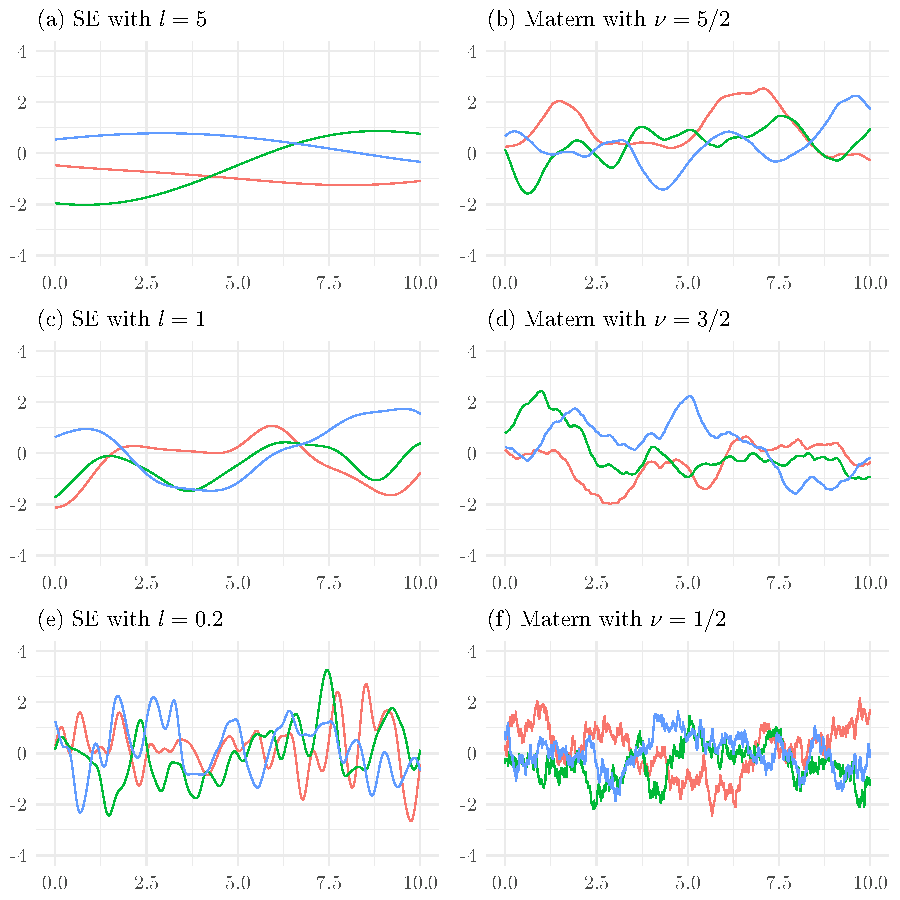
\includegraphics[scale=0.9]{fig2i.pdf}
\caption{Six plots, each with three samples from a zero-mean GP. Amplitude is $\sigma_f^2 = 1$ for each plot. In the plots (b), (d) and (f) with Matérn kernel, the length-scale $l = 1$. Variation in the length-scale of the Matérn kernel would have the same effect as in the squared exponential kernel, which is shown in plots (a), (c) and (e).} \label{fig:2i}
\end{figure}

\subsection{Automatic relevance determination}

Both of the above squared exponential and Matérn kernels are called \textit{stationary} as they are functions of $x - x'$. This means that they are invariant to transformations in the input space and corresponds to the modelling assumption that the objective function varies uniformly across the domain.

Further, since they are also both functions of $\lvert \x - \x' \rvert$ they are called \textit{isotropic} - uniform in all directions. However, this is often not the case and it would be advantageous to allow the kernel to express different rates of variation in different dimensions. More general \textit{anisotropic} kernels may be defined by replacing $\lvert \x - \x' \rvert^2$ by
%
\begin{equation}
r^2(\x, \x') = (\x - \x')^T D (\x - \x')
\end{equation}
%
for some positive semi-definite matrix $D$. Of course if $D$ is a dense (non-sparse) matrix it introduces many hyper-parameters, which may be difficult to deal with. As such, a popular choice for $D$ is a diagonal matrix with entries $D_{j,j} = 1/l_j^2$ such that:
%
\begin{equation}
r^2(\x, \x') = \sum_{j=1}^{d} \frac{(x_j - x'_j)^2}{l_j^2} \label{ard}
\end{equation}
%
The $l_j$ are simply individual length-scale hyper-parameters for each dimension. Kernels which are functions of equation \ref{ard} are called \textit{automatic relevance determination} kernels \cite{neal1996bayesian} as they allow for the relative importance of each dimension to be learned when the kernel hyper-parameters are tuned. This is helpful in dealing with cases where the objective function has low effective dimensionality, as was briefly mentioned in section \ref{sampledesigns}.

\section{Sampling from a Gaussian process}

Consider that we are interested in sampling from a zero-mean GP at a finite collection of points $\x_{1:n} := \{\x_1, \ldots, \x_n\}$, where each $\x$ is in $\D$. Since each $\x$ is itself a vector, any finite vector of indices induces a matrix which we denote by $X := [\x_1, \ldots , \x_n]^T \in \D^n \subseteq \mathbb{R}^{n \times d}$. The vector of random variables $\f := f(X) := [f(\x_1), \ldots , f(\x_n)]^T$ corresponding to this matrix by definition has a joint multivariate Gaussian distribution.

The parameters of this distribution are determined by applying the mean and kernel functions: $\f$ has mean vector $\B{0}$ and covariance matrix $K := k(X,X)$ with elements $K_{i,j} = k(\x_i,\x_j), \forall i=1, \ldots, n, j=1, \ldots, n$. The requirement that the kernel $k$ is positive-definite precisely means that any such matrix $K$, sometimes called the Gram matrix, is a valid covariance matrix. So, the distribution of $\f$ is:
%
\begin{equation}
\colvec{4}{f(\x_1)}{f(\x_2)}{\vdots}{f(\x_n)} \sim \N \left(
\colvec{4}{0}{0}{\vdots}{0}, 
\begin{bmatrix} k(\x_1, \x_1) & k(\x_1, \x_2) & \ldots & k(\x_1, \x_n) \\ 
				k(\x_2, \x_1) & k(\x_2, \x_2) & \ldots & k(\x_2, \x_n) \\
				\vdots        & \vdots        & \ddots & \vdots        \\
				k(\x_n, \x_1) & k(\x_n, \x_2) & \ldots & k(\x_n, \x_n) \\ 
\end{bmatrix}
\right)
\end{equation}
%
Put more succinctly:
\begin{equation}
\f \sim \N(\B{0}, K) \label{eq:ml}
\end{equation}
%
This distribution is referred to as the marginal likelihood, as it implicitly marginalizes out all possible function values at every $\x \in \D$ which is not in $\x_{1:n}$ \cite{duvenaud2014automatic}. This is justified by property \ref{itm:g1} of the multivariate Gaussian. For this reason, although a GP is an infinite object it is only ever necessary to consider finite subsets. Discretizing the domain and using equation \ref{eq:ml} allows us to visualize samples from a GP, as in figure \ref{fig:2i}.

Although this all does not seem particularly useful as it stands, shortly we will show that this distribution may be used as a prior in order to perform inference directly in function-space. It is for this reason that the notation $\mu_0$ is chosen for the prior mean function. First, however, we will take a brief interlude to discuss Bayesian linear regression and how it relates to GPs.

\section{Bayesian linear regression} 

Given a training data-set of observations and a new vector $\x_* \in \mathbb{R}^d$ of input variables, the aim of \textit{regression} is to predict target variable $f(\x_*)$. This is described as a \textit{supervised learning} task as the training data-set, i.e. the values of the target variable at the collection of inputs $\x_{1:n}$, plays the role of teaching us about the behaviour of $f$ \cite{sm3}. 

The approach of linear regression is to define a model in terms of a linear combination of fixed basis functions:
%
\begin{equation}
f(\x) = \B{w}^T\phi(\x)
\end{equation}
%
where $\B{w}^T$ is a vector of weights and $\phi(\x)$ is a vector of $M$ fixed non-linear basis functions that depend on the input vector $\x$. Many choices of basis functions are possible such as polynomial, Gaussian, sigmoidal or Fourier \cite{christopher2006pattern}. 

Typically the values of $\B{w}$ are estimated by minimizing the sum of squares error from the fitted values to the training data, which corresponds to finding the maximum likelihood estimator. This has analytic solution $\hat{\B{w}}$ given by the normal equations \cite{christopher2006pattern}
%
\begin{equation}
\hat{\B{w}} = \left(\B{\Phi}^T\B{\Phi}\right)^{-1}\B{\Phi}^T\f
\end{equation}
% 
where $\B{\Phi}$ is the design matrix with elements $\Phi_{n, k} = \phi_k(x_n)$ such that:
%
\begin{equation}
\B{\Phi} = 
\begin{pmatrix}
 \phi_1(\B{x}_1) & \phi_2(\B{x}_1) & \cdots & \phi_M(\B{x}_1) \\
 \phi_1(\B{x}_2) & \phi_2(\B{x}_2) & \cdots & \phi_M(\B{x}_2) \\
 \vdots  & \vdots  & \ddots & \vdots  \\
 \phi_1(\B{x}_n) & \phi_2(\B{x}_n) & \cdots & \phi_M(\B{x}_n) 
\end{pmatrix}
\end{equation}
%

A more Bayesian approach to this problem would be to place a prior distribution, say a Gaussian, on the weights $\B{w}$ such that:
%
\begin{equation}
p(\B{w}) = \N(\B{w} | \B{0}, \B{\Sigma}_w)
\end{equation}
%
where $\B{\Sigma}_w$ is the $M$ by $M$ covariance matrix. Notice that fixing $\B{w}$ fixes $f(\x)$, thus the probability distribution over $\B{w}$ induces a probability distribution over functions $f(\x)$. This distribution over functions is exactly a GP prior. As $f(\x)$ is a linear combination of Gaussian distributions it is itself Gaussian. The mean function $\mu_0$ is zero, as
%
\begin{align}
\nonumber \mu_0(\x) &= \E[f(\x)]  \\
\nonumber           &= \phi(\x) \E[\B{w}] \\
                    &= 0
\end{align}
%
and the covariance function is given by
%
\begin{align}
\nonumber k(\x, \x') &= \Cov(f(\x), f(\x')) \\
\nonumber            &= \E[f(\x)f(\x')] \\
\nonumber		     &= \phi(\x)^T \E[\B{w}^T\B{w}] \phi(\x') \\
		             &= \phi(\x)^T \Sigma_w \phi(\x')
\end{align}

This GP is called \textit{degenerate} precisely because it can be represented with a finite collection of basis functions as we have shown above. In fact, by Mercer's theorem, for every valid kernel function there exists a (possibly infinite) expansion in terms of basis functions \cite{rasmussen}. For example, taking $l^2 = \sigma_f^2 = 1$, the squared exponential kernel in one-dimension is given by \cite{vafa2016training}
%
\begin{align}
\nonumber k(x, x') = e^{- \frac{(x - x')^2}{2}} &= e^{-\frac{x^2}{2}}e^{-\frac{x'^2}{2}}\sum_{k=0}^{\infty} \frac{(xx')^k}{k!} \\
&= \phi(x)^T \phi(x')
\end{align}
where we have the infinite basis expansion
\begin{equation}
\phi(x) = e^{- \frac{(x - x')^2}{2}}\left[ 1, x, \frac{x^2}{\sqrt{2}}, \frac{x^3}{\sqrt{6}},... \right]
\end{equation}

\section{Gaussian process regression}

In this section we will show how regression can be done directly with GPs, \textit{without} having to think about the basis functions.

Suppose that at inputs $\x_{1:n}$ the values of the GP $\f = [f(\x_1), \ldots , f(\x_n)]^T$ are observed. We are interested in the value of the GP $f_* := f(\x_*)$ at a new input $\x_*$. By the GP definition, the joint prior distribution of $\f$ and $f_*$ is
%
\begin{equation} \label{eq:joint}
\colvec{2}{\f}{f_*} \sim \N \left(
\colvec{2}{\B{0}}{0},
\begin{bmatrix} K & k(X,\x_*)^T \\ 
				k(X,\x_*) & k(\x_*,\x_*) \\
\end{bmatrix} \right)
\end{equation}
%
where $k(X,\x_*) = [k(\x_1, \x_*), \ldots, k(\x_n, \x_*)]^T$ is the vector of covariance terms between the locations $\x_{1:n}$ and $\x_*$. For brevity this will in future be denoted by $\B{k}_*$. Now we make use of property \ref{itm:g2} of the multivariate Gaussian to find that the conditional distribution of $f_*$ given $\f$ is Gaussian
%
\begin{equation}
f_* \vert \f \sim \N(\mu_n(\x_*), \sigma^2_n(\x_*))
\end{equation}
%
with mean and variance given by
%
\begin{align} 
\mu_n(\x_*) &= \B{k}_*^T K^{-1} \f \label{eq:predmean} \\ 
\sigma^2_n(\x_*) &= k(\x_*,\x_*) - \B{k}_*^T K^{-1} \B{k}_* \label{eq:predvar}
\end{align}
%
This is known as the \textit{predictive distribution} as it gives the mean and variance at any given unobserved test point $\x_*$. 

Often, it is not possible to directly observe $\f$ itself.  Instead, we may observe a noise contaminated version $\y$, where each $y = f(\x) + \epsilon$ as in property \ref{itm:p4}. We assume Gaussian additive independent identically distributed noise with zero mean and variance $\sigma^2$ such that:
\begin{equation}
p(\y \vert \f) = \N(\y \vert \f, \sigma^2I)
\end{equation}
%
Integrating out the unobserved values $\f$ with distribution $p(\f)$ from equation \ref{eq:ml}, the marginal likelihood is:
%
\begin{align} \label{eq:mln}
p(\y) &= \int d\f \, p(\y|\f)p(\f) \\
      &= \N(\y \vert \B{0}, K + \sigma^2I) 
\end{align}
%
Introducing the additional noise term to \ref{eq:joint}, the joint distribution of the values $\y$ and $f_*$ is:
%
\begin{equation}
\colvec{2}{\y}{f_*} \sim \N \left(
\colvec{2}{\B{0}}{0},
\begin{bmatrix} K + \sigma^2I & \B{k}_*^T \\ 
				\B{k}_* & k(\x_*,\x_*) \\
\end{bmatrix} \right)
\end{equation}
%
This can be conditioned as before to show that the predictive distribution $p(\f_* \vert \y)$ is Gaussian with mean and variance given by:
%
\begin{align} \label{eq:npredmean}
\mu_n(\x_*) &= \B{k}_*^T(K + \sigma^2I)^{-1}\y \\
\sigma^2_n(\x_*) &= k(\x_*,\x_*) - \B{k}_*^T(K + \sigma^2I)^{-1}\B{k}_* \label{eq:npredvar}
\end{align}
%
Taking $\sigma^2 = 0$ recovers equations \ref{eq:predmean} and \ref{eq:predvar}. The predictive distribution actually defines a posterior Gaussian process in its own right \cite{snelson2008flexible} with mean function as in equation \ref{eq:npredmean} and kernel function
%
\begin{equation}
k(\x, \x') = k(\x,\x') - \B{k}^T(K + \sigma^2I)^{-1}\B{k}'
\end{equation}
%
where $\B{k} = [k(\x_1, \x), \ldots, k(\x_n, \x)]^T$ and $\B{k}'$ is defined similarly.

Observe that rather than depending on a fixed number of parameters, the complexity of the model adapts to the number of training data points \citep{orbanz2011bayesian}. As such, GP regression is an example of a Bayesian \textit{non-parametric} model, where the parameter-space is infinite. This is advantageous as we do not have to specify a parametric structure and have less worries about over-fitting, which in parametric modelling typically must be combated with regularization.

In equation \ref{eq:predmean} notice that that predictive mean is simply a linear combination of the of the observations. For this reason equation \ref{eq:predmean} is known as a linear predictor \cite{rasmussen} - in fact it is actually the best linear unbiased predictor \cite{lectures}.

In equation \ref{eq:npredvar} the predictive variance is the prior variance minus a (positive) term which only depends on the training data locations. The closer the training data locations $\x_{1:n}$ are to $\x_*$ the greater the values in the vector $\B{k}_*$ are, and the greater the Mahalanobis distance $\B{k}_*^T(K + \sigma^2I)^{-1}\B{k}_*$. This explains the visual effect, which can be seen in figure \ref{fig:2i}, of the predictive variance decreasing closer to the training data points. That being said, it may be considered disappointing that the predictive variance is completely independent of the actual values observed $\y$: surely if an unexpected value is observed then this should be accounted for by increased uncertainty. \citet{shah2014student} for this and other reasons propose the use of the more general Student-t process as an alternative to the GP.

\begin{figure}
\centering
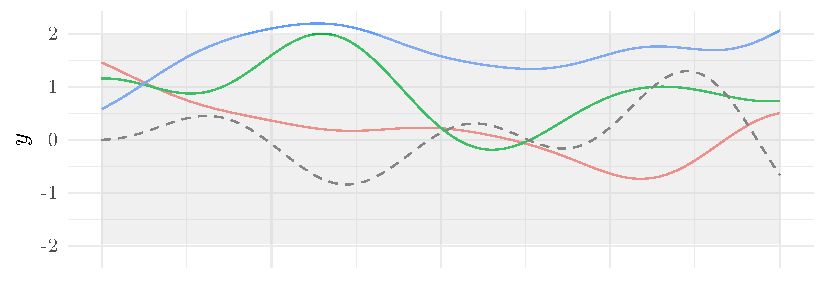
\includegraphics[scale=1]{fig2iia.pdf}
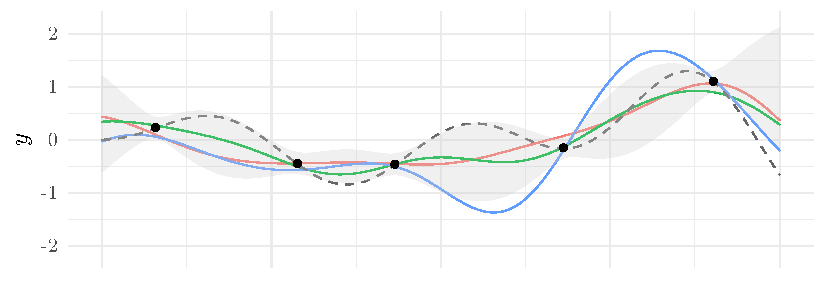
\includegraphics[scale=1]{fig2iib.pdf}
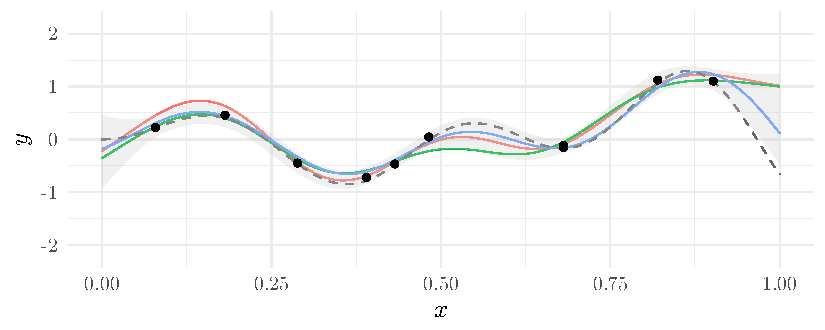
\includegraphics[scale=1]{fig2iic.pdf}
\caption{GP regression example. In each plot there are three samples curves from a GP with with prior mean zero and  squared exponential kernel with hyper-parameters $\param = (\sigma_f, l) = (1, 0.15)$. Data is generated by objective function $f(x) = \sin(5x)\sin(13x)\exp(x-0.5)$, shown as the grey dotted line, with additive Gaussian noise with variance $\sigma^2 = 0.01$. The shaded region is a $95\%$ confidence interval calculated using the predictive mean \ref{eq:npredmean} and variance \ref{eq:npredvar} equations.} \label{fig2ii}
\end{figure}

The dimension of the matrix $K$ is the number of data points observed $n$. This matrix is inverted in equations \ref{eq:predmean} and \ref{eq:predvar} usually by computing the Cholesky decomposition. This has computational cost big $\mathcal{O}(n^3)$, which is typically the bottleneck of GP regression - limiting it's reach to relatively small $n$. This has motivated the development of sparse Gaussian processes \cite{quinonero2005unifying} \cite{snelson2006sparse} which approximate the posterior over functions to make inference computationally cheaper.

\section{Learning the hyper-parameters} \label{sec:modelselection}

In the complete hierarchical Bayesian model selection framework \cite{mackay1992bayesian} models are specified in three tiers: model parameters, model hyper-parameters and model structures. We will focus our attention on model selection at the second level, the model hyper-parameters.

At the bottom level the model parameters are obtained by the posterior distribution over functions, as our model is non-parametric. The top level corresponds to the choice of kernel function, which is one of the key challenges of GP regression. To alleviate potential problems, the kernel functions chosen are purposefully flexible as we have discussed. 

This leaves the model hyper-parameters, which are the hyper-parameters of the kernel function $\param$ together with the noise-variance $\sigma^2$ if it is unknown. The most simplistic approach would be to specify the hyper-parameters a-priori, however ill-fitting choices, illustrated in figure \ref{fig:2iii}, can lead to very poor performance. As a result it is better to learn the hyper-parameters from the data, which may be done by maximizing the marginal likelihood, which is analytic for GP models and given by equation \ref{eq:mln}. Making the dependence of $K$ on the kernel hyper-parameters $\param$ explicit, its logarithm is:
%
\begin{align} \label{eq:loglike}
\nonumber \log p(\y \vert X, \param) = 
&-\frac{n}{2}\log2\pi 
\underbrace{-\frac{1}{2}\log\lvert K_{\param} + \sigma^2I \rvert}_{\text{controls model capacity}} \\
& \underbrace{- \frac{1}{2} \y^T(K_{\param} + \sigma^2I)^{-1}\y}_{\text{encourages fit with data}}
\end{align}
%
Optimizing this likelihood gives an empirical Bayes estimate for the hyper-parameters. Equation \ref{eq:loglike} balances the trade-off between fit and complexity of the model \cite{duvenaud2014automatic}. The second term penalizes the complexity of the model as the determinant of the covariance matrix grows with more complicated kernels, such as those with  smaller length-scales. The final term is a Mahalanobis distance which controls the quality of the fit.

\begin{figure}
\centering
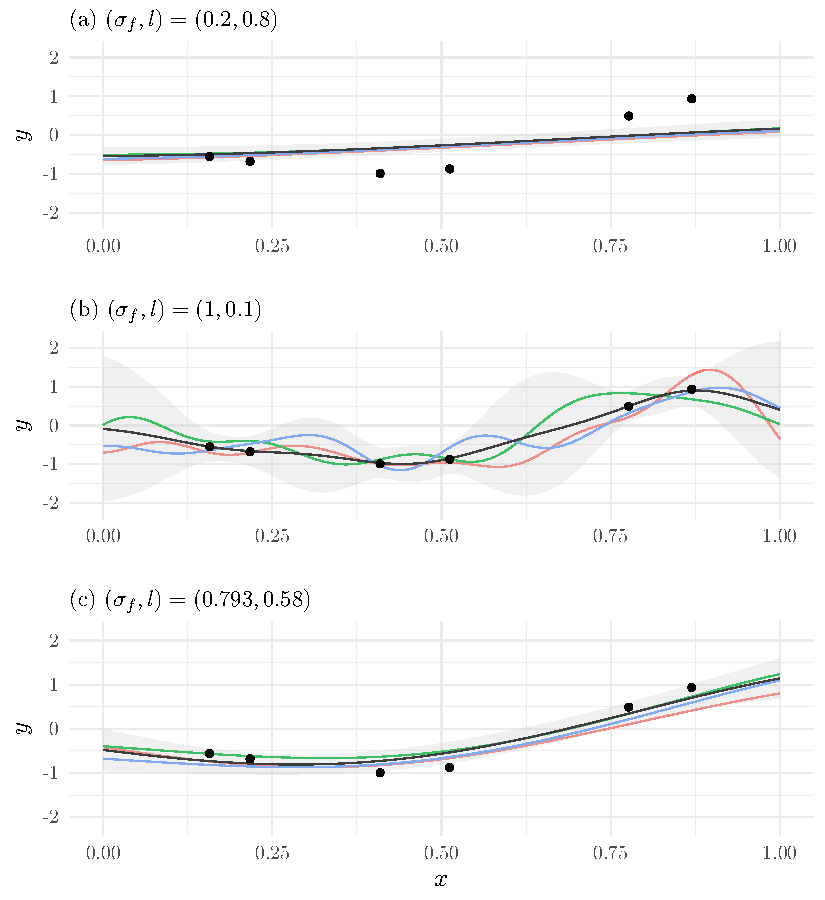
\includegraphics[scale=1]{fig2iii.pdf}
\caption{The impact of different amplitude and length-scale hyper-parameters on squared exponential kernel GP regression models. As in figure \ref{fig2ii} there are three sample curves with the addition of a black mean function. Figure (a) is an example of under-fitting the data. It is overly simplistic and fails to capture the underlying trend in the data. Figure (b) is an example of over-fitting. It is a more complex model which has mean function that interpolates the data. Finally, figure (c) uses the maximum likelihood estimates of the hyper-parameters and is a balance between figures (a) and (b).} \label{fig:2iii}
\end{figure}

There are many possible ways to optimize equation \ref{eq:loglike}. One alternative is to use quasi-Newton methods such as the Broyden–Fletcher–Goldfarb–Shanno (BFGS) algorithm with random restarts. In this project we will use the L-BFGS-B algorithm \cite{byrd1995limited} which approximates the BFGS algorithm and is adapted to handle simple box-constraints on the hyper-parameters, i.e. bounded above and below. This algorithm is used in many R implementations of GP regression such as the \texttt{DiceKriging} \cite{roustant2012dicekriging}, \texttt{GPfit} \cite{macdonald2013gpfit} and \texttt{laGP} \cite{gramacy2016lagp} packages.

In Bayesian optimization, the hyper-parameters are typically tuned at every iteration of the algorithm - in particular whenever a GP is fit. 
% Chapter 3

\chapter{Acquisition functions} % Main chapter title

\label{Chapter3} % For referencing the chapter elsewhere, use \ref{Chapter3} 

%----------------------------------------------------------------------------------------

In sequential optimization, the next point in the search space to be evaluated at each stage is determined by an optimization \textit{policy} $\bm{\pi}$ which is a sequence of decision rules $\pi_n$ which map from the space of possible training data at stage $n$ to a point $\x_n \in \D$. In Bayesian optimization a GP emulator to the objective function fit on all the data available at stage $n$ is used to help inform this decision. 

How should the policy $\bm{\pi}$ be chosen?

\section{Optimal policies}

A natural place to start is to look for a policy which is in some sense optimal. In order to find such a policy it is necessary to define a metric so that performance can be measured. The loss function regret \citep{sugden} is a sensible choice \cite{srinivas2009gaussian} for this metric. We define the \textit{instantaneous regret} at stage $n$ as the difference between the (potentially unknown) immediate reward of the optimal action $f(\x^\star)$ and the actual immediate reward received $f(\x_n)$, so that
%
\begin{equation}
r_n = f(x_n) - f(\x^\star)
\end{equation}
%
The \textit{cumulative regret} $R_N = \sum_{n=1}^{N} r_n$ is the sum of instantaneous regrets at each stage. \textit{Simple regret} is the instantaneous regret of the final recommendation $x^-$ of the algorithm. 

Different varieties of regret are appropriate to different situations. Cumulative regret is a sensible way to measure performance in online problems such as the multi-armed bandit problem, which we introduced in section \ref{sec:bandits}. In off-line problems however there is no need to penalize poor performance during the optimization process as this would discourage exploration. Simple regret instead should be considered.

As the optimization is stochastic, the optimal policy minimizes the \textit{expectation} of the simple regret. Unfortunately, such a policy is the solution to an dynamic programming problem which requires solving many nested maximizations and expectations \cite{lam2016bayesian} and is therefore intractable. Although there has been some recent work \cite{gonzalez2015glasses} \cite{lam2016bayesian} in this area, the majority of the focus has instead been on more tractable policies defined by so-called acquisition functions.

\section{Acquisition functions}

Acquisition functions provide a heuristic, typically myopic, measure of the utility of prospective query points. At stage $n$ to determine the next point to query $\x_{n}$, the chosen acquisition function $\alpha$ is maximized over the design space.
%
\begin{equation} \label{eq:acquistion}
\x_n = \argmax_{\x\in\mathcal{X}} \alpha(\x)
\end{equation}
%
In other words, the optimization policy $\bm{\pi}$ is, in a way, homogenized - each decision rule $\pi_n$ is replaced with the consultation of a particular acquisition function. That being said, although it has been omitted in equation \ref{eq:acquistion} the acquisition function may depend on the stage $n$, in some way.

Many possible acquisition function have been suggested in the literature. The chosen acquisition function should effectively balance the trade-off between local and global search. To encourage local search it should be high where the posterior predictive mean is low and to encourage global search it should be high where the posterior predictive marginal variance is high.

A common approach is to look for points which offer improvement over some incumbent value $\nu \in \D$, which represents the best solution found so far\footnote{Notation has been overloaded: unrelated to the smoothness parameter of the Matérn kernel}. This value $\nu$ is typically the minimum function evaluation observed so far 
%
\begin{equation}
\nu = \min \{f(\x_1), \ldots, f(\x_{n-1}) \}
\end{equation}
%
when observations are deterministic, or the minimum expected value of the emulator 
%
\begin{equation}
\nu = \argmin_{\x\in\D} \mathbb{E}[f(\x)]
\end{equation}
%
when the objective function is noisy \citep{lizotte}. We will discuss two improvement-based acquisition functions, probability of improvement and expected improvement, in the following sections \ref{sec:pi} and \ref{sec:ei}.

\subsection{Probability of improvement} \label{sec:pi}

Early work by \citet{kushner1964new} proposes maximizing the probability that $f(\x)$ improves on the incumbent, $\nu$. This may be calculated analytically by noting that at stage $n$ the random variable $f(\x)$ has Gaussian distribution with mean and variance given by predictive equations \ref{eq:predmean} and \ref{eq:predvar}. The GP emulator has has been conditioned on the data-set $\Da_{n-1}$, but for ease-of-exposition we will denote this mean and variance simply by $\mu(\x)$ and $\sigma(\x)$ respectively. As such, the \textit{probability of improvement} (PI) acquisition function is
%
\begin{equation}
\alpha_\mathrm{PI}(\x) \equiv \mathbb{P}(f(\x) \leq \nu)
= \Phi\left(\frac{\nu - \mu(\x)}{\sigma(\x)}\right)
= \Phi(z(\x))
\end{equation}
%
where $\Phi(\cdot)$ is the standard normal cumulative distribution function and $z(\x) = {(\nu - \mu(\x))}/{\sigma(\x)}$ is the standardization score.

The drawback of this approach is that global search is often neglected because likely improvements, however infinitesimal, are favoured \cite{brochu2010interactive}. The search will move on, but only after almost exhaustively fine-tuning the current best solution. To remedy this, Kushner proposes that the minimum improvement accepted is a trade-off parameter $\xi(n)$. His idea being that $\xi(n)$ operates on a cooling schedule, starting high to encourage global search and decreasing towards zero later so that solutions are refined locally. \citet{jones2001taxonomy} describes that although performance may be impressive, the method is extremely sensitive to the choice of this parameter.

\subsection{Expected improvement} \label{sec:ei}

\textit{Expected improvement} (EI) \citep{mockus1974bayesian} is another natural, improvement-based, approach which overcomes some of the drawbacks of PI. As well considering the probability that $f(\x)$ improves on $\nu$, EI also takes into account the degree of that potential improvement. In particular, under the model, the improvement function $\mathrm{I}(\cdot)$ is defined to be the random variable
%
\begin{equation}
\mathrm{I}(\x) \equiv \max \{0, \nu - f(\x)\}
\end{equation}
%
The likelihood of attaining improvement $I > 0$ is simply Gaussian, with density
%
\begin{equation}
\frac{1}{\sqrt{2\pi}\sigma(\x)} \textrm{exp} \left \{ -\frac{1}{2} \frac{(\nu - I - \mu(\x))^2}{\sigma^2(\x)} \right \}
\end{equation} 

Taking the expected value of the improvement over this density gives the expected improvement acquisition function
%
\begin{equation}
\alpha_{\mathrm{EI}}(\x)
\equiv \E[ \mathrm{I}(\x) ] 
= \int_0^\infty I \, \frac{1}{\sqrt{2\pi}\sigma(\x)} \textrm{exp} \left \{ -\frac{1}{2} \frac{(\nu - I - \mu(\x))^2}{\sigma^2(\x)} \right \} \, dI
\end{equation}
%
Using integration by parts \citep{schonlau1996global} this expression has the closed form
%
\begin{equation} \label{eq:ei}
\alpha_{\mathrm{EI}}(\x) = \sigma(\x)[z(\x)\Phi(z(\x)) + \phi(z(\x))]
\end{equation}
%
where $\Phi(\cdot)$ is as before and $\phi(\cdot)$ is the standard normal probability density function. 

EI has attractive theoretical convergence properties \citep{bull2011convergence} and has been shown to work well in practice \citep{snoek2012practical}, for example as a part of the ``Efficient Global Optimization'' algorithm \citep{jones1998efficient}. Further, it is easy to implement and does not require setting any additional parameters. For these reasons it is often the default choice. 

\subsection{Lower confidence bound}

Originally studied in the the multi-armed bandit setting by \citet{lai1985asymptotically}, the \textit{lower confidence bound} (LCB) acquisition function \cite{srinivas2009gaussian} is an optimistic acquisition function which assumes a fixed probability best-case scenario occurs, and looks for the point which is best under this scenario. It is defined to be:
%
\begin{equation}
\alpha_{\mathrm{LCB}}(\x) \equiv \lambda\sigma(\x) - \mu(\x)
\end{equation}
%
The constant $\lambda$ is used to to explicitly balance between local search and global search by setting this fixed probability. \citet{srinivas2009gaussian} are able to show that with appropriate choice of $\lambda$ as a function of $n$ the LCB acquisition function is what is called no-regret, which means that $\lim_{N\to\infty} R_N / N = 0$, with high probability.

\section{Maximizing the acquisition function} \label{maxacq}

By using an acquisition function, the primary optimization problem \ref{eq:1.1} has been traded for a series of optimization problems \ref{eq:acquistion}: one for each stage. For this trade to be viable it must be easy to optimize the acquisition function. Thankfully unlike the objective function the acquisition functions all have analytic expressions which can be sampled cheaply.

Various approaches have been proposed and successfully implemented in the literature. Most simplistically, the domain can be discretized and exhaustively grid-searched - which is of course how visualizations like figure \ref{fig:1ii} are produced. In this project we will use the same algorithm as was used to optimize the GP hyper-parameters - namely L-BFGS-B with random restarts.
% Chapter 4

\chapter{Constrained optimization} % Main chapter title

\label{Chapter4} % For referencing the chapter elsewhere, use \ref{Chapter4} 

%----------------------------------------------------------------------------------------

\section{Introduction}

Previously we considered the optimization problem in equation \ref{eq:1.1} where all values $\x$ in the search space $\mathcal{X}$ are valid. In constrained optimization problems this is not the case: there are a set of additional requirements, called \textit{constraints}, that $\x$ must meet for it to be considered feasible. Using a set of $K$ inequality constraints $c_k : \D \to \mathbb{R}$ this may be formulated as the constrained optimization problem:
%
\begin{equation} \label{eq:cop}
\x^\star = \argmin_{\x\in\mathcal{X}} f(\x)\quad
\mathrm{s.t.}\quad c_k(\x) \geq 0, \forall k \in \{1,...,K\}
\end{equation}
%
The set of points $\x$ which satisfy each of the constraints $c_k$ is called the \textit{feasible region} $\mathcal{R}\subseteq\mathcal{X}$. Points outside the feasible region are called \textit{infeasible}.

Constraints may be of two types, \textit{coupled} or \textit{decoupled}. Coupled constraints may only be evaluated jointly alongside the objective function. That is, when the objective function has been queried the user also learns the value of the constraint function. Decoupled constraints, on the other hand, can be evaluated independently of the objective. This is more of a challenge since if each constraint is decoupled then at every stage there is a choice of $K+1$ functions (the $K$ constraints plus the the objective function $f$) which may be queried.

We consider that, in general like the objective function, the constraints are: not necessarily linear or convex \ref{itm:p1}; black-box \ref{itm:p2}; and expensive to evaluate individually \ref{itm:p3} in the decoupled case. In addition, the constraints may be noisy \ref{itm:p4}, which will be discussed in section \ref{sec:nconst}. Without these properties, it may be possible to cheaply find the feasible region $\mathcal{R}$ and to proceed with unconstrained optimization on this reduced search space.

The addition of constraints considerably widens the scope of problems which may be considered compared with the unconstrained case. Returning to a previous example, when optimizing the hyper-parameters of a machine-learning model there may be settings which cause the model to diverge, so the optimization may need to be constrained. Other examples include optimizing CPU speed of a processor whilst restricting power usage below some threshold or optimizing the yield of a chemical process whilst limiting the amount of unwanted by-products which are produced. 

Some authors \cite{gardner2014bayesian} \cite{letham2017constrained} also present constrained optimization as a proxy method for dealing with trade-offs. In their paper about optimizing systems at Facebook, \citet{letham2017constrained} state that:
%
\begin{quotation}
`` ...there are almost always trade-offs involved in optimizing real systems: improving the quality of images may result in increased data usage; increasing cache sizes may improve the speed of a mobile application, but decrease reliability on some devices; optimizing click-through rates may result in decreases in quality.''
\end{quotation}
%
In general, these problems may perhaps more generally be described as multi-objective optimization problems in which the output $\y$ has dimension greater than one. Of course there is no strict ordering for points in $\mathbb{R}^2$ and above, and so the aim of multi-objective optimization is to approximate the Pareto set of non-dominated points \cite{dt3}. For example, a more complete treatment of a chemical yield optimization with constrained unwanted by-products may find the highest yield possible for any given acceptable amount of by-product. The simplification is possible because constrained optimization is a special case of  multi-objective optimization, in which the constraint functions are treated as objective functions which are constant over the feasible region and negative infinity elsewhere \cite{gelbart}.  

\subsection{Noisy constraints} \label{sec:nconst}

Problems where evaluations of the constraints are contaminated by noise are particularly challenging. If it is assumed that the noise is Gaussian then no point, even if directly observed many times, can be guaranteed to be feasible. As such, the constrained optimization problem formulated in equation \ref{eq:cop} is ill-posed: it is impossible to know with certainty that any of the constraints have been met. 

It is reasonable instead to require that each constraint $c_k$ is met with high-probability \cite{gelbart}. We define the $k$th Boolean \textit{probabilistic constraint} $\mathcal{C}_k$ such that
%
\begin{equation}
\mathcal{C}_k(\x) \quad \iff \quad \mathbb{P}(c_{k}(\x)\geq 0) \geq 1 - \delta_k
\end{equation}
%
for some confidence level $\delta_k$. The condition that each of the $K$ probabilistic constraints $\mathcal{C}_k$ are met is denoted $\mathcal{C}$ such that: 
%
\begin{equation}
\mathcal{C}(\x) \quad \iff \quad \forall k, \, \mathcal{C}_k(\x)
\end{equation}
%
Now, the noisy constrained optimization problem is:
%
\begin{equation} \label{eq:ncop}
\x^\star = \argmin_{\x\in\mathcal{X}} f(\x)\quad
\mathrm{s.t.}\quad \mathcal{C}(\x)
\end{equation}
%
Notice that equation \ref{eq:cop} may be recovered by requiring certainty of satisfying the constraints, that is by setting $\delta_k = 0$ for all $k$.

\section{Constrained Bayesian optimization}

Bayesian optimization is a promising strategy for constrained optimization problems. For example, the dissertation of Griffiths \citep{griffiths} uses constrained Bayesian optimization to optimize the molecular properties of drug candidates, using constraints to avoid invalid molecular structures.

The plan is to model each of the constraints $c_k$ by GP emulators - which are sequentially updated as data is observed, just as we have done with the objective function. For tractability, the emulators are assumed to be conditionally independent given the input $\x$. Now the only alteration that needs to be made is to in some way incorporate the constraints into the acquisition function. We will discuss two ways of doing this.

\subsection{Expected improvement with constraints}

Expected improvement, introduced in section \ref{sec:ei}, may be extended to consider the equation \ref{eq:cop} where the constraints are coupled. This was first proposed by \citet{schonlau1998global} and has been revisited more recently \cite{snoek2013bayesian} \cite{gardner2014bayesian} - in particular by \citet{gelbart} who extends it to the equation \ref{eq:ncop}. 

The main idea is to assign zero improvement to all infeasible points and to adjust the incumbent value $\nu$ to either be the best point observed to be feasible so far or the minimum of the posterior mean such that $\mathcal{C}(\nu)$ is true. 

Proceeding similarly to the unconstrained case, the constrained improvement function is the random variable
\begin{equation}
\mathrm{I}_C(\x) \equiv \mathrm{max}\{0, \nu - f(\x)\} \, \Delta(\x)
\end{equation}
%
where $\Delta(\x) \in \{0, 1\}$ is the constraint indicator function - taking value 1 if each of the constraints are met and 0 otherwise. Taking the expectation as before gives the \textit{constrained expected improvement} (EIC) acquisition function, which we are able to factor due to the assumed conditional independence given $\x$ of the emulators:
%
\begin{align}
\nonumber \alpha_{\mathrm{EIC}}(\x) &\equiv \mathbb{E}[ \mathrm{max}\{0, \nu - f(\x)\} \, \Delta(\x) \, \vert \, \x ] \\
\nonumber                 &= \mathbb{E}[\mathrm{max}\{0, \nu - f(\x)\} \, \vert \, \x] \, \mathbb{E}[\Delta(\x) \, \vert \, \x] \\ 
                          &= \alpha_{\mathrm{EI}}(\x)\prod_{k=1}^{K} \mathbb{P}(c_{k}(\x) \geq 0)
\end{align}
%
Notice that this is easily interpretable as a product of the unconstrained expected improvement function and the probability of satisfying each of the constraints. Applying the closed form from equation \ref{eq:ei} and noting that $\mathbb{P}(c_{k}(\x) \geq 0)$ is a Gaussian CDF we have
%
\begin{equation}
\alpha_{\mathrm{EIC}}(\x) = \sigma(\x)[z(\x)\Phi(z(\x)) + \phi(z(\x))] \prod_{k=1}^{K} \Phi\left( \frac{\mu_k(\x)}{\sigma_k(\x)} \right)
\end{equation}
%
where $z(\x) = {(\nu - \mu(\x))}/{\sigma(\x)}$ as before and the predictive mean and standard deviation of constraint $k$ are given by $\mu_k(\x)$ and $\sigma_k(\x)$. Due to this analytic form, EIC is easy to implement.

\citet{gelbart} points out that this formulation is inconsistent when no feasible point has been observed (that is there does not exist a point $\x$ such that $\mathcal{C}(\x)$ holds) and proposes that in this case the algorithm should focus all its attention on locating a such a point:
\begin{equation}
\alpha_{\mathrm{EIC}}(\x) = 
\begin{cases} 
\, \alpha_{\mathrm{EI}}(\x)\prod_{k=1}^{K} \mathbb{P}(c_{k}(\x) \geq 0), &\mbox{if } \exists \x \, \mathrm{s.t.} \, \mathcal{C}(\x) \\ 
\, \prod_{k=1}^{K} \mathbb{P}(c_{k}(\x) \geq 0), & \mbox{otherwise } 
\end{cases}
\end{equation}



\subsection{Integrated expected conditional improvement}

The EIC acquisition function is structured to avoid sampling infeasible points, but it may be beneficial to sample such points in order to provide information in the long run. This drawback is a symptom of the wider myopia of expected improvement. To remedy this \citet{gramacy2011optimization} propose using a so-called \textit{integrated expected conditional improvement} (IECI) acquisition function. IECI is also improvement-based like EI, but is designed to have additional look-ahead to help it make better long-term decisions. 

In particular, rather than being based on the improvement function, IECI is based on the conditional improvement function $\mathrm{I}(\cdot\mid\cdot)$. It is a measure of the improvement at a reference point $\x'$ after a candidate point $\x$ has been chosen to be sampled, but not yet evaluated:
%
\begin{equation} \label{eq:conditionalimprovement}
\mathrm{I}(\x' \mid \x) \equiv \max \{0, \nu - f(\x' \mid \x)\}
\end{equation}

GP models are not dynamic, and so the distribution of $f(\x' \mid \x)$ remains $f(\x')$ prior to the observation at $\x$. However, it is in fact possible to deduce what the predictive variance of the updated model will be once that observation has happened. Recall that the predictive variance equation \ref{eq:npredvar} is not dependent on the actual values observed $\y$, only the training data locations $\x_{1:n}$. Following this observation, \citet{gramacy2011optimization} \textit{define} the distribution of $f(\x' \mid \x)$ to be Gaussian with predictive mean $\mu(\x')$ conditioned on the data actually observed and predictive variance $\sigma^2_\x(\x')$ conditioned on the data actually observed together with the unobserved $\x$. The closer $\x'$ is to $\x$ the greater the reduction in predictive variance, assuming that the kernel function is concave. Therefore, taking the expectation of equation \ref{eq:conditionalimprovement} simply amounts to replacing $\sigma^2(\x')$ in equation \ref{eq:ei} by $\sigma^2_\x(\x')$
%
\begin{equation}
\mathbb{E}[\mathrm{I}(\x' \mid \x)] = \sigma_\x(\x')[z(\x')\Phi(z(\x')) + \phi(z(\x'))] \label{eq:expectedci}
\end{equation}
%
where $z(\x') = {(\nu - \mu(\x'))}/{\sigma_\x(\x')}$. 

Taking a step back for a second, remember that we are looking for an acquisition function which can be maximized as a function of $\x$ only. For this reason we first integrate over the reference point $\x' \in \D$, with arbitrary well-behaved distribution $g(\x')$. Secondly, notice that we prefer candidate points which \textit{minimize} expected conditional improvement, for example by reducing $\sigma_\x(\x')$ in equation \ref{eq:expectedci}. As a result we negate the integral to give a general IECI acquisition function, defined to be:
%
\begin{equation}
\alpha_{\mathrm{IECI}}(\x) \equiv - \int_{\x' \in \D} \mathbb{E}[\mathrm{I}(\x' \mid \x)] g(\x') \; d\x' \label{eq:ieci}
\end{equation}

Rather than think of minimizing the expected conditional improvement, it is perhaps more intuitive to think of maximizing the expected reduction in improvement. Speaking heuristically, the amount of improvement in a system is finite and should decrease with each additional observation, reaching zero when a minimizer $\x^\star$ is found. Choosing candidate points $\x$ which maximize this reduction should lead to an efficient optimization policy. 

These two approaches are analogous. To make the connection clear, we use the fact that acquisition functions can scaled additively without changing the maxima - and therefore leading to the same decision making in practise. Since $\mathbb{E}[I(\x')] g(\x')$ is entirely independent of $\x$ we may rescale equation \ref{eq:ieci} to give the equivalent integrated expected reduction in improvement (IERI) acquisition function:
%
\begin{align}
\nonumber \alpha_{\mathrm{IERI}}(\x) &\equiv 
\int_{\x' \in \D} \mathbb{E}[I(\x')] g(\x') \; d\x' - \int_{\x' \in \D} \mathbb{E}[\mathrm{I}(\x' \mid \x)] g(\x') \; d\x' \\
&= \int_{\x' \in \D} \left( \mathbb{E}[I(\x')] - \mathbb{E}[\mathrm{I}(\x' \mid \x)] \right) g(\x') \; d\x' \label{ieri}
\end{align}

This is all well and good, but we still have the problems of dealing with the distribution $g(\x')$ and incorporating the constraints. However, the IECI acquisition function is built to be able to deal naturally with both these problems at once. This is accomplished by using the density $g(\x')$ to favour reductions in expected improvement in regions likely to be feasible. In particular, taking $g(\x')$ to be the probability of satisfying each of the $K$ black-box constraints $c_k$ gives the constrained IECI acquisition function:
%
\begin{equation}
\alpha_{\mathrm{IECI}}(\x) \equiv - \int_{\x' \in \D} \mathbb{E}[\mathrm{I}(\x' \mid \x)] \prod_{k=1}^{K} \mathbb{P}(c_{k}(\x') \geq 0) \; d\x' \label{cieci}
\end{equation}
%
This is the form of IECI that we will use in this project. One drawback is that this integral is not tractable in general and is instead approximated \cite{gramacy2011optimization}.
 
% Chapter 5

\chapter{Experiments} % Main chapter title

\label{Chapter5} % For referencing the chapter elsewhere, use \ref{Chapter4} 

%----------------------------------------------------------------------------------------

The two-dimensional Branin-Hoo function is often used as a bench-mark for optimization \cite{eggensperger2013towards} \cite{picheny2013benchmark}. For our experiments, we use a deterministic version \cite{sfu} rescaled to the unit square $[0,1]^2$ with
%
\begin{equation} \label{eq:branin}
f(\x) = \frac{1}{51.95} \left[ (\bar{x}_2 - \frac{5.1}{4\pi^2}\bar{x}_1^2 + \frac{5}{\pi}\bar{x}_1 - 6)^2 + 10(1-\frac{1}{8\pi}\cos(\bar{x}_1)) - 44.81 \right] 
\end{equation} 
%
where $\bar{x}_1 = 15x_1 - 5$ and $\bar{x}_2 = 15x_2$. This rescaled version has mean zero and variance one. It is a multi-modal function with global minima $-1.047$ at three locations: $(0.124, 0.818)$, $(0.543, 0.152)$ and $(0.962, 0.165)$, to three decimal places.

\section{Unconstrained} \label{experiment1}

To demonstrate the capability of Bayesian optimization we first optimize the unconstrained Branin-Hoo function. 

The optimization budget is taken to be $N = 20$ function evaluations. An initial dataset $\Da_0$ of five points is generated by latin-hypercube sampling (LHS), leaving fifteen iterations to be selected by the chosen acquisition function.

\begin{figure}
\centering
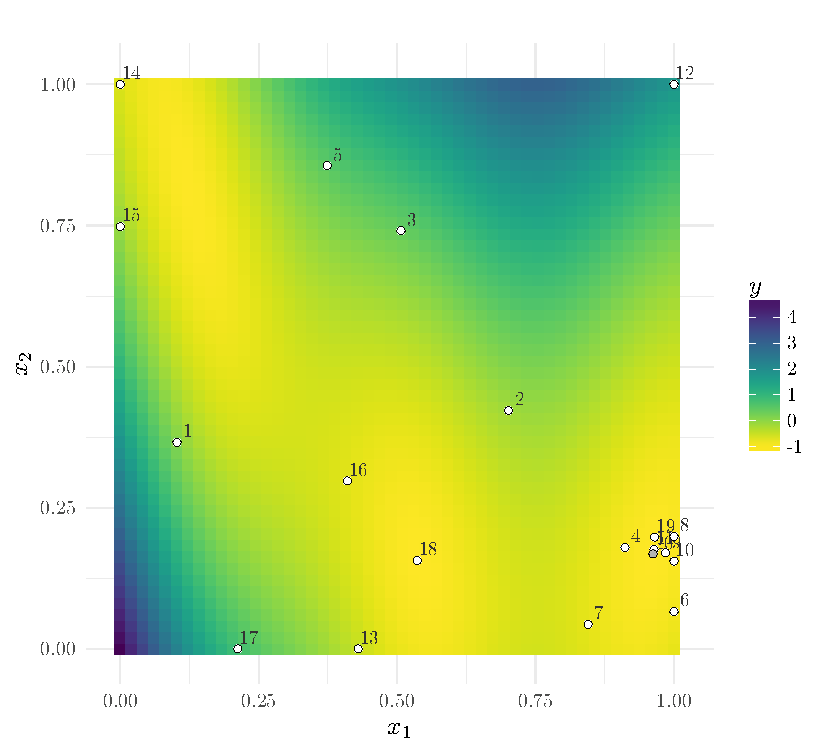
\includegraphics[scale=1]{fig5i.pdf}
\caption{Density plot of modified Branin-Hoo function, as specified by equation \ref{eq:branin}. Example numbered Bayesian optimization path plotted as white circles. Points one to five are generated by latin-hypercube sampling and points six to twenty are chosen by maximizing EI acquisition function. Minimum sample location, shown as the grey circle, is the final point $(0.965, 0.198)$ with value $-1.043$ to three decimal places.} \label{fig:5i}
\end{figure}

The implementation of is written in R using the \texttt{laGP} \cite{gramacy2016lagp} package, based on the lecture notes of \citet{lectures}. For simplicity an isotropic squared exponential kernel is used. To ease computation the prior mean function $\mu_0$ of the GP is set to be zero and the amplitude $\sigma_f^2$ of the kernel is set to be one. The length-scale $l$ of the kernel is tuned at each iteration of the algorithm to be the maximum likelihood estimator. The acquisition function used is expected improvement with incumbent value $\nu$ set to be the minimum function value observed so far. One benefit of choosing EI is that it does not require any additional parameters, such as the constant $\lambda$ for LCB. Both the optimization of the log-likelihood, given by equation \ref{eq:loglike}, and the optimization of the acquisition function are performed using five random restarts of \texttt{method="L-BFGS-B"} via the default function \texttt{optim}.

\begin{figure}
\centering
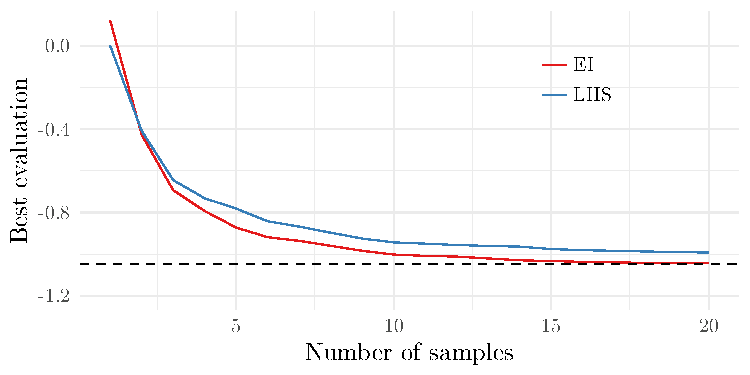
\includegraphics[scale=1]{fig5ii.pdf}
\caption{The progress, averaged over 50 runs, of both EI and LHS. Recall that the first five points chosen by both methods are by LHS, so the variation for these samples is due to randomness. However from that point onwards it is clear that EI convincingly converges on the true global minimum -1.047, shown by the horizontal dashed line, whereas LHS makes comparatively slow progress.} \label{fig:5ii}
\end{figure}

Figure \ref{fig:5i} shows the result of one run of the Bayesian optimization procedure, which we henceforth refer to as EI, described above. Of course the results of any single run are not statistically significant because the first five samples locations, together with the starting locations of the log-likelihood and acquisition function optimization procedures, are random.  

To average out some of the variation we repeat the EI procedure independently 50 times. To provide a baseline for comparison we also run 50 repeats where all 20 points are chosen by LHS. Figure \ref{fig:5ii} compares the average performance of each procedure. It is clear that the performance of EI in this instance is superior: 29 out of the 50 times EI finds a global minimum to three decimal places compared to only once out of 50 for LHS. 

\section{Constrained} \label{experiment2}

Similarly to the set-up in \citet{gelbart} and Griffiths \cite{griffiths} we now consider as before the optimization the Branin-Hoo function, but now with the additional, deterministic, black-box disk constraint $c(\x) \geq 0$, where:
%
\begin{equation}
c(\x) = \frac{2}{9} - (x_1 - \frac{1}{2})^2 - (x_2 - \frac{1}{2})^2
\end{equation}
%
This constraint excludes points outside a circle of radius $\sqrt{2}/3$ centred at $(0.5, 0.5)$. Of the three global minimizers of the unconstrained objective function, two now lie outside the feasible region, leaving only one feasible global minimizer, $(0.543, 0.152)$. It is assumed that the constraint is coupled, so that $f$ and $c$ are evaluated jointly.

We will test the performance of the two constrained optimization acquisition functions introduced in Chapter \ref{Chapter4}, EIC and constrained IECI, together with LHS. As before, the optimization budget is $N=20$ and the first five iterations of each method are chosen by LHS. 

In both the EIC and IECI implementations the constraint, like the objective function, is modelled by a GP with squared exponential kernel and the incumbent value $\nu$ is set to be the minimum function value observed so far. Whereas EIC is entirely tractable, the integral in IECI is approximated by a sum weighted by the probability of satisfying the constraint. For this reason IECI was substantially more computationally demanding.

Figure \ref{fig:5iii} illustrates the region which is now infeasible due to the constraint and shows an example EIC optimization path. Figure \ref{fig:5iv} shows the surrogate functions to the objective and constraint functions, respectively, after the 20 points in the previous figure have been sampled. In this specific instance it is clear that the surrogates are well fitted to both the objective and constraint.

Overall, across 50 repeats, we find that EIC performs slightly better than IECI, with both performing much better than LHS. In particular, the average of the minimum feasible function evaluations found is -1.037 for EIC, -1.032 for IECI and -0.966 for LHS. This is shown by figures \ref{fig:5v} and \ref{fig:5vi}. 

\begin{figure}
\centering
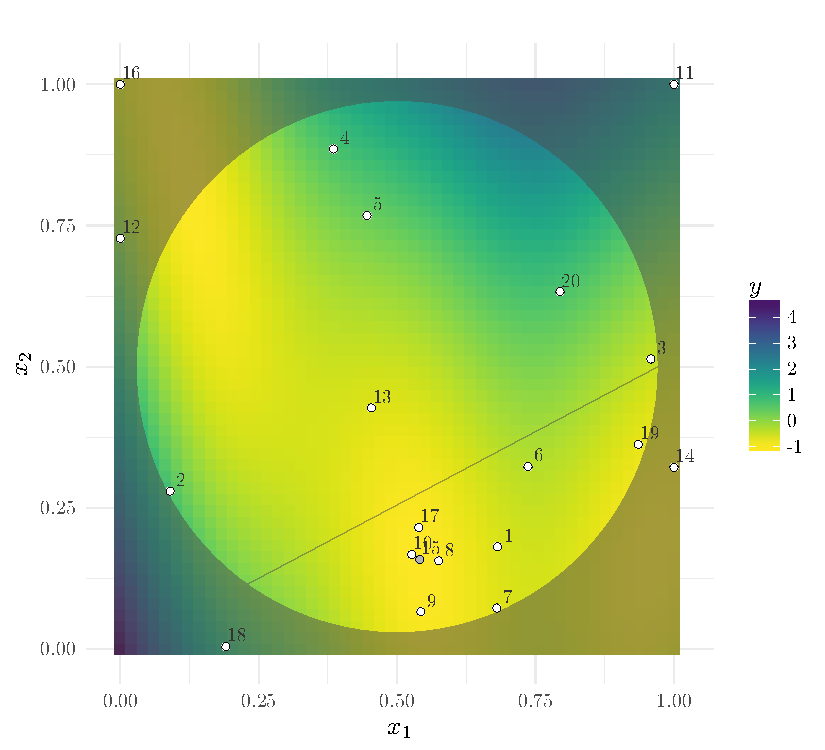
\includegraphics[scale=1]{fig5iii.pdf}
\caption{As in figure \ref{fig:5i} a density plot of Branin-Hoo function is shown. The region which is infeasible, that is $c(\x) < 0$, is shaded in a darker colour. The white circles show a numbered example EIC optimization path, with the grey circle showing minimum feasible sample location $(0.541, 0.158)$ with value -1.047 to three decimal places. In this instance EIC is able to find the one feasible global minimizer. It is interesting to note samples 11, 12, 14, 16 and 18 are taken close to the edge of the unit square.} \label{fig:5iii}
\end{figure}

\begin{figure}
\centering
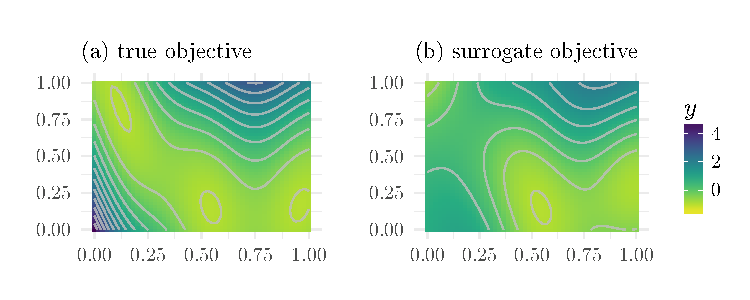
\includegraphics[scale=1]{fig5iva.pdf}

\vspace{-20pt}

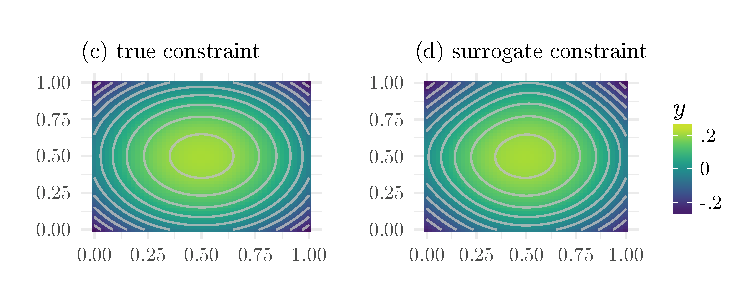
\includegraphics[scale=1]{fig5ivb.pdf}
\caption{
Plots (a) and (b) show the true objective function and the mean of its GP emulator after the 20 points in figure \ref{fig:5iii} have been sampled. To allow for meaningful comparison, they have been rescaled to a common colour scale. Although the surrogate is overall a good fit, it misses the minimizer in the top left. This corresponds to the fact that there are no samples in that location in figure \ref{fig:5iii}. It is also instructive to note that the surrogate function does not fit well in regions where the objective function is high, and that this is not a bad thing. We are only interested in accurately learning the objective function in regions where it may plausibly have a global minimizer.
% 
Similarly, plots (c) and (d) show the true constraint function and the mean of its GP emulator after the 20 samples in figure \ref{fig:5iii}, on a common colour scale (which is oppositely oriented, because we are looking for positive constraint values). The surrogate is very similar to the true constraint, perhaps due to the constraints simplicity.} 
\label{fig:5iv}
\end{figure}

\begin{figure}
\centering
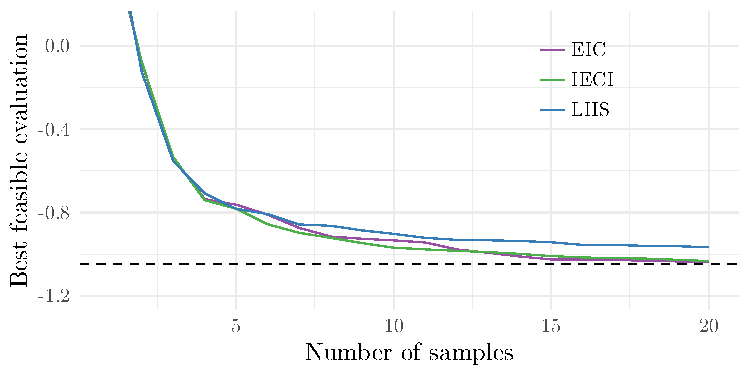
\includegraphics[scale=1]{fig5v.pdf}
\caption{The progress, averaged over 50 runs, of the EIC, IECI and LHS implementations. As in figure \ref{fig:5ii} the true global minimum -1.047 is shown by the horizontal dashed line.} 
\label{fig:5v}
\end{figure}

\begin{figure}
\centering
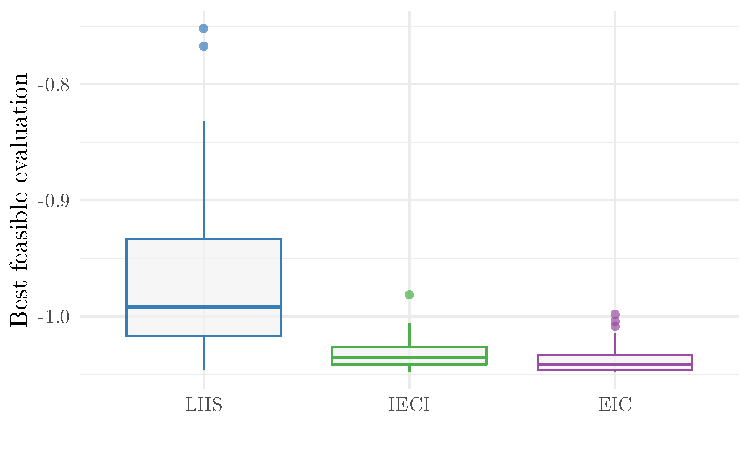
\includegraphics[scale=1]{fig5vi.pdf}
\caption{Boxplot of the best feasible evaluation found after 20 samples for each method, across the 50 runs.} 
\label{fig:5vi}
\end{figure}

One explanation for why EIC may have outperformed IECI in this particular problem is because of the simplicity of the constraint. In particular, there is not much that can be learned from sampling in the infeasible region as the global minimizer is a fair distance from it. Perhaps IECI may prove its value for problems with more complicated feasible regions. Another explanation is that the IECI implementation is only an approximation: it may be that the true version would perform better. This is plausible because a previous implementation of IECI was run with a faster, less accurate, approximation which averaged only -1.017.

\section{Discussion}

These results show the promise of Bayesian optimization and that the algorithm works essentially as hoped, for both unconstrained and unconstrained optimization problems. Of course from a critical point of view there are some caveats which should be mentioned. 

Firstly, in both the constrained and unconstrained cases, the Bayesian optimization implementations are in some sense unfairly helped by the objective function being scaled to have mean zero and variance one, as they have not had to learn these facts from the data.

The Branin-Hoo function is not a particularly difficult optimization problem. As all of the local minimizers are global so there is no threat of placing too great an emphasis on local search. That being said, there is circumstantial evidence of a balanced approach in figures \ref{fig:5i} and \ref{fig:5iii}. Furthermore, it is only two-dimensional which, while being convenient for visualisation, is not particularly demanding. One current challenge is scaling Bayesian optimization to be more effective in higher dimensions, as for the time being it is restricted to roughly 10 dimensions \cite{wang2016practical}.

Furthermore, both the objective and constraint are taken to be deterministic. Had property \ref{itm:p4} been the case the results surely would have been less impressive. Problems with high noise-levels are particularly challenging and can lead to odd, pathological, behaviour if not considered more thoroughly \cite{gelbart} \cite{letham2017constrained}.

Finally, it almost goes without saying that we have only tested performance on one specific function - more rigorous benchmarks should test on a variety of objective functions.






% Chapter 6

\chapter{Conclusion} % Main chapter title

\label{Chapter6} % For referencing the chapter elsewhere, use \ref{Chapter4} 

%----------------------------------------------------------------------------------------

In Chapter \ref{Chapter1} we began by introducing four properties of the objective function and the challenges they pose to optimization. Via discussion of three sample design strategies we presented some of the prominent considerations, principles and trade-offs in such a problem. This motivated a sequential, model-based approach - known as Bayesian optimization. 

Chapter \ref{Chapter2} explores Gaussian process emulators to the objective function, which are the most commonly used statistical model for Bayesian optimization. We discussed some of the design challenges, such as the choice of kernel function and handling of hyper-parameters, in the practical implementation of GPs. Chapter \ref{Chapter3} explains the role of the acquisition function and gives three examples. Our first experiment, in section \ref{experiment1}, demonstrated the application of this theory, resulting in a substantial performance improvement on LHS.

We have also considered the extension of Bayesian optimization to deal with black-box, inequality constraints. Chapter \ref{Chapter4} introduces two constrained acquisition functions, expected improvement with constraints and integrated expected conditional improvement, which are tested against each other in our second experiment, section \ref{experiment2}. The results of this experiment seem to suggest that for simple feasible regions EIC may be preferable to IECI - quite how plausible such simplistic feasible regions are in practice is questionable. 

The discussion of constrained Bayesian optimization was by no means exhaustive: two suggestions for further study are the work of \citet{gramacy2016modeling} on augmented Lagrangian approaches and the work of \citet{hernandez2015predictive} on so-called predictive entropy search with constraints.

Needless to say, there is still a great deal of work to be done on Bayesian optimization. A look at last years NIPS workshop \cite{nips} gives an idea of the direction moving forward: scaling to larger data-sets, moving beyond GPs and making the overall Bayesian optimization toolbox more comprehensive and easy to use. A great deal of this work is directly driven by problems in science and engineering and as such there is a lot of room for collaboration. A number of companies have also been founded aiming to use provide Bayesian optimization as a service \cite{osborne2018}. This all goes to say that it is a dynamic and exciting research area to be a part of. 

  

%----------------------------------------------------------------------------------------
%	THESIS CONTENT - APPENDICES
%----------------------------------------------------------------------------------------

\appendix % Cue to tell LaTeX that the following "chapters" are Appendices

% Include the appendices of the thesis as separate files from the Appendices folder
% Uncomment the lines as you write the Appendices

%% Appendix A

\chapter{Gaussian identities} % Main appendix title

\label{AppendixA} % For referencing this appendix elsewhere, use \ref{AppendixA}

Let $\x$ be a $d$ dimensional vector with multivariate Gaussian distribution 
%
\begin{equation}
[\x_1, \x_2]
\end{equation}

%\include{Appendices/AppendixB}
%\include{Appendices/AppendixC}

%----------------------------------------------------------------------------------------
%	BIBLIOGRAPHY
%----------------------------------------------------------------------------------------

\printbibliography[heading=bibintoc]

%----------------------------------------------------------------------------------------

\end{document}  
